\chapter{Les biographies de Muḥammad, Prophète de l'islam}

Après avoir abordé le milieu religieux de la péninsule arabique à l'aube
du VIIe siècle, et distingué à grands traits les grandes dates de la
naissance de l'islam, il convient à présent de focaliser notre attention
sur celui qui est considéré par les musulmans comme le messager de la
Révélation coranique, Mahomet ou Muḥammad \TArabe{ (مُحَمَّد)}. Personnellement,
j'écris Muḥammad qui est la translittération du nom du Prophète de
l'arabe en français, tandis que Mahomet est l'écriture francisée, venant
du latin Mahometus. Que sait-on de lui~? Comment vivait-il~? À quelle
religion appartenait-il~? A-t-il fréquenté des juifs, des chrétiens et
des mazdéens de La Mecque~? Comment sa prédication a-t-elle été reçue~?
Quand parvient-il à imposer la légitimité de sa mission~? Comment s'y
prend-il~? Quelles relations entretient-il avec son clan~? Sa tribu~?
Était-il prophète, roi et chef de guerre, comme on le dit~?

Les questions sont posées. Elles sont importantes. J'en pose une autre,
au préalable~: Comment fait-on pour savoir~? Comment s'y prend-on pour
répondre~? En historien, on s'appuie forcément sur des sources, en
portant sur elles un regard critique, et ce d'autant plus que la
première «~biographie~» de Muḥammad date de la fin du VIIIe
siècle\ldots{} donc du temps des abbasides. Le temps a passé, il y a
déjà eu l'ère des califes bien guidés, les Rashidūn (cela a donné le
prénom Rashid, au féminin~: Rashida), puis celui de l'empire des
Omeyyades. Si vous ne voyez pas qui sont les califes bien guidés,
relisez le chapitre 2. Or, écrire une biographie n'est jamais neutre.

Certes, une lecture croyante peut fort bien vouloir se dispenser des
études critiques sur les fondations de l'islam, mais comme l'écrit
l'historien tunisien Hichem Djaït dans la biographie qu'il consacre à
Muḥammad~: 
\begin{quote}
  «~la science est une, et le souci de scientificité est la
marque des sociétés libres~»\sn{Hichem Djaït, La vie de Muḥammad,
  Volume 2, Paris, Fayard, 2008 p. 13.}.  
\end{quote}


\paragraph{les Sources} Il me semble donc incontournable de consacrer quelques pages du cours à
la question épistémologique : de quelles sources disposons-nous~? Quel
est leur statut~?

Mais la question des sources posées, il faut constater que la figure
même de Muḥammad a donné lieu à de multiples biographies au cours des
siècles. C'est le pluriel qui s'impose. Certes, il y a les premières
grandes biographies dont la matrice est donnée par Ibn Iṣḥāq
\TArabe{
(ابن
إسحاق)}, mais au cours des siècles va se développer des images de
Muḥammad et cela jusqu'à nos jours. Quelles sont ces images~?

Dans ce chapitre sur les fondations de l'islam, il nous semble opportun
de donner aussi quelques passages de ces premières biographies. À cet
égard, je m'appuierai sur les textes de la Sīra d'Ibn Hishām, car c'est
la plus populaire. Le préambule méthodologique permettra aussi
d'analyser ces informations~dans les contextes politiques et religieux
où elles ont été données.


\paragraph{{La question méthodologique~: comment écrire la biographie de Muḥammad~? }}

En arabe, la biographie de Muḥammad s'appelle Sīra. Aujourd'hui, les
biographies du Messager de l'islam ne manquent pas. En français, il y a
celles écrites par des musulmans à l'exemple d'Al-Sira de Mahmoud
Hussein -- pseudonyme commun de Bahgat Elnadi et Adel Rifaat,
politologues français d'origine égyptienne --, de Tariq Ramadan,
Muhammad, La vie du Prophète ou encore de l'historien tunisien Hichem
Djaït, La vie de Muḥammad, écrite en trois volumes parus en français aux
éditions Fayard et que nous avons déjà cité ci-dessus.

On trouve aussi celles des orientalistes comme Maxime
Rodinson\sn{Maxime Rodinson, Mahomet, Paris, 1956.}, Tor
Andrae\sn{Tor Andrae, Les Origines de l'islam et le christianisme,
  tr. fr., Paris, 1955.}\textsuperscript{,} Régis Blachère, W.
Montgommery Watt\sn{Montgomery Watt, Mahomet à La Mecque~; Mahomet
  à Médine, trad. Fr., Paris, 1958 et 1959.}, Jacqueline Chabbi et son
livre {Le Seigneur des tribus}. La dernière en date de ce point de
vue est celle écrite par l'orientaliste allemand Tilman Nagel. Les
approches entre les biographies confessantes et les biographies
historiques sont bien sûr différentes, très différentes. Mais il faut
bien voir que pour les musulmans, la biographie n'est pas une écriture
a-historique. Au contraire, la biographie du Prophète est
intrinsèquement liée à celle de l'histoire de la naissance de l'umma. Il
s'agit d'approcher Muḥammad, son univers culturel, mais aussi social.
Les historiens musulmans ont le souci de rendre compte des moindres
personnages ayant fréquenté Muḥammad, mais aussi de ses gestes
quotidiens. Tarif Khalidi dans {Images of Muḥammad} dit qu'avec la
Sīra, c'est un peu comme si on avait voulu retranscrire le nom des 5 000
personnes venues écouter le Sermon sur la montagne de Jésus. Ce genre de
biographies de la première communauté s'appelle les {Tabaqāt}.
C'est un genre littéraire typique de l'islam. Par ailleurs, si dans les
Évangiles, on sait peu de choses de la vie privée de Jésus, la Sīra
aborde aussi bien la vie publique que la vie privée et intime de
Muḥammad\sn{Tarif Khalidi, Images of Muḥammad. Narratives of the
  Prophet in Islam. Across the Centuries, New York, Doubleday, 2009.}.

Dans un article paru dans la revue {History Compass} en 2007,
Robert Hoyland présente les différents points de vue et méthodologies
mises en œuvre en vue de dessiner un portrait authentique de
Muḥammad\sn{Robert Hoyland, «~Writing the Biography of the Prophet
  Muḥammad~: Problems and Solutions~», History Compass, 5/2, 2007, p.
  581-602.}. Dans tous les cas, l'intention est la même~: se rapprocher
de la réalité.

Hoyland souligne dans un premier temps que l'image du Prophète Muḥammad
qui est véhiculé du côté occidental a d'abord été négative~: Muḥammad
(ou ceux qui se revendiquent de son message) conquiert des terres et
impose une religion en portant un message qui au final nie la divinité
du Christ. On va y voir un homme d'ambition et de passion, au pire la
figure de l'Antéchrist, le fils du diable. L'époque médiévale applique
la parole de Jésus sur les faux prophètes. Dans la {Somme contre
les Gentils} Saint Thomas d'Aquin avance les preuves rationnelles de
l'impossibilité pour Muhammad d'être dit «~prophète~» :
\begin{quote}
    «~Par
  contre, il {[}Mahomet{]} a entremêlé les vérités de son enseignement
  de beaucoup de fables et de doctrines les plus fausses. Il n'a pas
  apporté de preuves surnaturelles, les seules à témoigner comme il
  convient en faveur de l'inspiration divine, à savoir quand une œuvre
  visible qui ne peut être que l'œuvre de Dieu prouve que le docteur de
  vérité est invisiblement inspiré. Il a prétendu au contraire qu'il
  était envoyé dans la puissance des armes, preuves qui ne font point
  défaut aux brigands et aux tyrans. ~Aucune prophétie divine ne
  témoigne en sa faveur : bien au contraire, il déforme les
  enseignements de l'Ancien et du Nouveau Testament par des récits
  légendaires, comme c'est évident pour qui étudie sa loi. Aussi bien,
  par une mesure pleine d'astuces, il interdit à ses disciples de lire
  les textes de l'Ancien et du Nouveau Testament qui pourraient le
  convaincre de fausseté.~»
\end{quote}
Au xvième, Luther dans un essai de 1528,
\sn{Luther, {De la guerre contre les Turcs} (Vom Kriege wider die Türken)}
expose l'incompatibilité de l'islam avec la foi chrétienne. Dans le
contexte de l'invasion ottomane en Europe et du Siège de Vienne, il
appelle à la résistance contre les turcs et, si Muḥammad ne peut
l'Antéchrist, puisque c'est le pape qui l'est, il ne peut donc être
qu'un «~démon~», le fruit du mensonge, celui qui fait table rase de la
vérité chrétienne, qui détruit «~l'ordre spirituel de la foi et de la
vérité~»\sn{Pour une étude sur l'islam chez Luther
  voir~: A.S Francisco, Martin Luther and Islam. A Study in
  Sixteenth-Century Polemics and Apologetics, coll. The History of
  Christian-Muslim Relations 8, Leiden, Brill, 2007.}. Cette vision est
encore celle du philosophe Pascal au xviie siècle.

Les lumières apportent un regard renouvelé sur l'islam qu'il s'agit
d'intégrer à une vision universelle de l'humanité, et au XIXème siècle,
d'une manière surprenante, Ernest Renan dans {Mahomet et les
origines de l'islamisme}, écrit~:
\begin{quote}
    «~La vie de son fondateur nous est aussi bien connue que celle de tel
réformateur du xvie siècle. Nous pouvons suivre année par année les
fluctuations de sa pensée, ses contradictions, ses faiblesses~».
\end{quote}


Cet optimisme repose sur l'assurance en l'authenticité des paroles et
gestes consignés par la tradition musulmane. Or, au \textsc{XIXème}
siècle, l'orientaliste Ignaz Goldziher est le premier à avoir, mis en
avant l'aspect reconstruit du {ḥadīṯ} et il concluait qu'il ne peut
constituer un matériel historique pour rendre compte de la naissance de
l'islam~; il permet cependant de mettre en lumière des tendances
dogmatiques ou juridiques qui se sont développées au cours des premiers
siècles. Henri Lammens \label{Theol:Lammens2} au début du XXème siècle publie en 1912
{Fatima et les filles de Mahomet}: {notes critiques pour
l'étude de la Sira}. Il montre que

\begin{quote}
    «~l'inspiration de la Sīra est d'abord exégétique. Dérivée en droiture
du texte du Qoran, la Sīra est destinée à lui servir de commentaire en
action~; elle doit traduire, en anecdotes précises et pittoresques, les
allusions les plus obscures, les sous-entendus les moins intelligibles
des versets, faire la chasse à l'anonyme, à l'impersonnel, si
déconcertants dans la lecture des sourates, partout, pour ainsi dire,
apposer des plaques commémoratives, multiplier la mention des noms
propres, les dates, si prudemment évités par Abou'l Qasim~» \label{Lammens1} \sn{Henri
  Lammens, Fatima et les filles de Mahomet: notes critiques pour l'étude
  de la Sīra, Rome, Institut Biblique Pontifical, 1912, p. vii.}.
\end{quote}


Bref, la Sīra doit combler l'obscurité du Coran, elle doit l'expliquer,
l'historiciser, mais elle vise aussi à préciser la doctrine coranique et
la jurisprudence. Ainsi, il existait parmi les juristes de Médine et
ceux de La Mecque et d'Irak, deux positions relatives à la possibilité
pour un pèlerin de contracter un mariage. De part et d'autre, la vie de
Muḥammad et ses paroles vont être convoquées pour fonder leur position,
quitte à ce qu'il y ait contradiction. Joseph Schacht conclut que bien
des éléments de la vie de Muḥammad, des détails importants, ne sont pas
fondés sur une recollection authentique mais sont fictifs et servent à
défendre des doctrines juridiques. L'articulation entre la vie du
Prophète et l'exégèse n'a pas perdu de son actualité~: c'est la
perspective de Patricia Crone~: «~Une grande partie de la tradition
apparemment historique est en fait d'origine exégétique~»\sn{Patricia
  Crone, Meccan Trade and the Rise of Islam, Oxford, 1987, p. 214.}.

De ces difficultés, certains orientalistes ont cherché à approcher
Muḥammad à partir du Coran seul. C'est le cas de Régis Blachère. Mais
cette approche est aussi celle de musulmans qu'on appelle les
\textbf{coranistes}~: pour eux, l'islam c'est le Coran et seulement le
Coran. Cependant, ce n'est pas sans difficulté car le Coran est peu
prolixe sur son environnement et à l'exception des noms bibliques, on ne
trouve que deux noms de personnages qui sont mentionnés~: celui de
Muḥammad, à quatre reprises, et celui d'Abū Lahab.


\paragraph{À propos d'Abū Lahab que l'on trouve dans la sourate 111, 1-5~: }
\begin{quote}
    Que périssent les deux mains d'Abū Lahab
et que lui-même périsse. Sa fortune ne lui sert à rien, ni ce qu'il a
acquis. Il sera brûlé dans un feu plein de flammes, de même sa femme, la
porteuse de bois, à son cou une corde de fibres.
\end{quote}


On apprend par les commentaires qu'il
s'agit de son oncle, hostile à Muḥammad et que la femme est surnommée la
porteuse de bois car elle jetait du bois et des plantes épineuses sur la
route qu'empruntait le Prophète\ldots{} mais sans les commentaires, le
Coran lui-même reste très énigmatique.


Le Coran fait aussi mention des Romains et de la tribu de Quraysh, mais
pas des autres tribus. Huit lieux sont indiqués, quatre communautés
religieuses (juifs, chrétiens, mages et sabéens) ainsi que trois
divinités arabes. Et si La Mecque est nommée, aucune indication sur son
rôle dans la vie de Muḥammad. Il est question dans le Coran de Badr mais
rien ne permet d'y voir une référence explicite à la fameuse bataille du
même nom, même si l'interprétation est possible.

 
\subsection{À propos de la bataille de
Badr} 

C'est la première grande bataille militaire que mène Muḥammad après son
exil à Médine contre une caravane de Mecquois. Une armée d'hommes
accompagnée de milliers d'anges vont emporter leur première victoire
contre les notables de La Mecque~; Muhammad y acquiert le prestige de
fin stratège.

Selon les commentaires coraniques, le Coran ferait allusion à cette
bataille~:




\begin{table}[h!]
\resizebox{\textwidth}{!}{%
\small
\begin{tabular}{p{7cm}p{7cm}}

Il y eut déjà pour vous un signe dans ces deux troupes qui
s'affrontèrent: l'une combattait dans le sentier d'Allah; et l'autre,
était mécréante. Ces derniers voyaient les croyants de leurs propres
yeux, deux fois plus nombreux qu'eux-mêmes. Or Allah secourt qui Il veut
de Son aide. Voilà bien là un exemple pour les doués de clairvoyance !
& 

\\

S. 3, 123~ Allah vous a donné la victoire, à Badr, alors que vous étiez humiliés.
Craignez Allah donc. Afin que vous soyez reconnaissants! &  
\TArabe{

وَلَقَدْ نَصَرَكُمُ اللَّهُ بِبَدْرٍ وَأَنتُمْ أَذِلَّةٌ فَاتَّقُوا
اللَّهَ لَعَل

َّكُمْ تَشْكُرُونَ }
\\

\end{tabular}%
}
 
\end{table}



 \begin{figure}
 \centering
 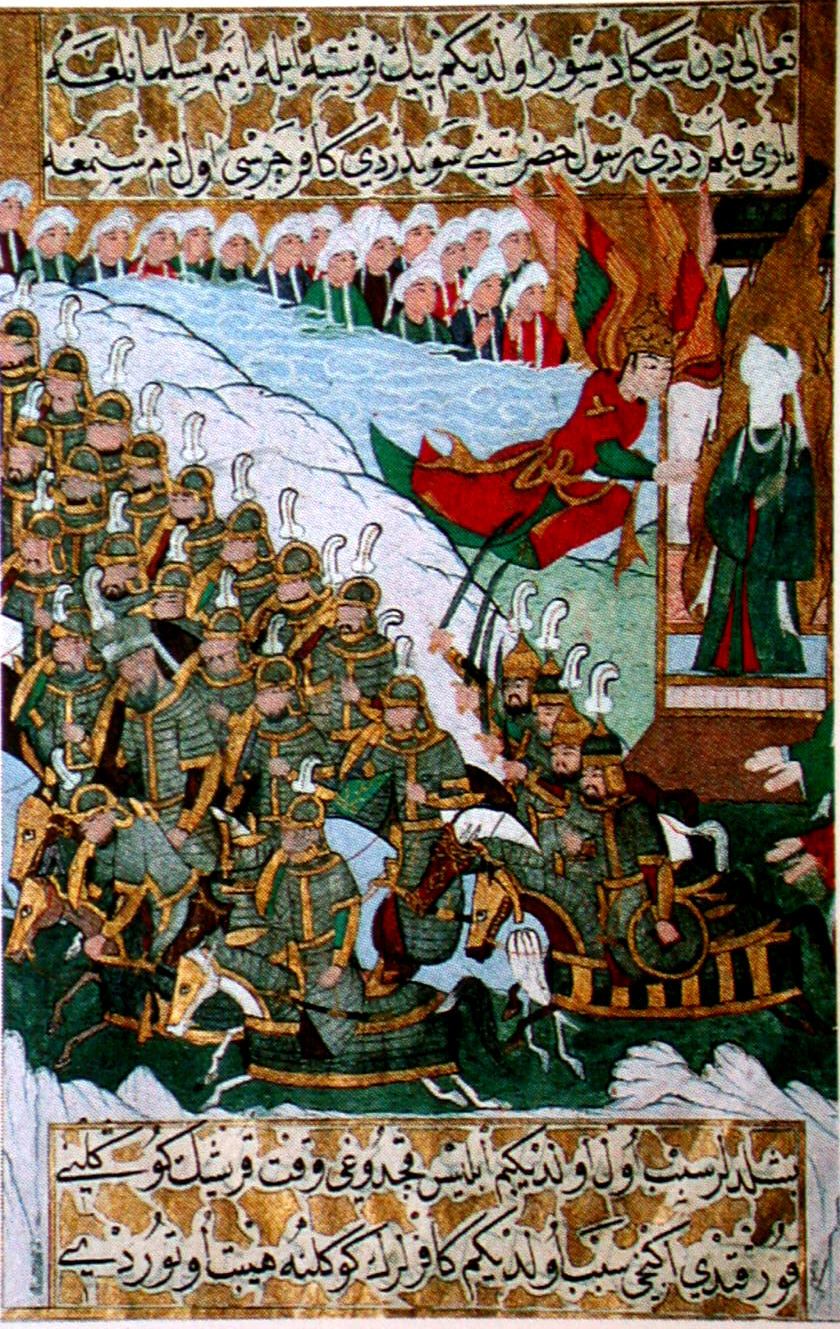
\includegraphics[width=0.5\textwidth]{Images/image038.jpg}
 \caption{La bataille de Badr S. 3, 13 et 123. Remarquez l'ange Gabriel qui annonce la
victoire à Muḥammad. Le visage du Prophète est voilé. Au milieu, entre les combattants, de l'eau : Badr est le
nom d'un puits d'eau. Pour Muḥammad il est en cela un lieu stratégique
dans la mesure où la caravane devra s'y
arrêter.}
 \label{fig:Badr}
 \end{figure}



Dans\textit{ De la guerre}, Carl von Clausewitz a dressé la théorie de
l'importance du puits d'eau dans le combat.

Dans ce contexte, Montgomerry Watt a réhabilité le matériel traditionnel
dans sa biographie de Muḥammad notamment tout ce qui a trait aux
expéditions militaires dans la mesure rien ne ces textes ne cherchent à
expliciter le Coran, le commenter, et que de la même manière il ne
s'agit pas de développements doctrinaux ou jurisprudentiels.

De ces avertissements, de ces difficultés, il s'ensuit que le biographe
de Muḥammad est pris entre deux tenailles~: à la fois il encourt le
risque de rejeter tout matériel historique comme étant une pieuse
invention ou d'intégrer à la réalité historique des éléments de légende
et des inventions. Et finalement, comme le dit Maxime Rodinson, on
risque d'écrire une biographie en fonction de ses propres intérêts,
questions, présupposés, intuitions, comme à l'époque de la tradition
musulmane.

Fort de ces difficultés, à laquelle s'ajoute une idéalisation de la
figure de Muḥammad comme guide à suivre et modèle à imiter, Tilman Nagel
a cherché à «~déchiffrer les conceptions religieuses~» de Muḥammad en
remontant au-delà des sources normatives. Il a utilisé des données de la
poésie, les sources extra-islamiques, l'histoire préislamique de La
Mecque et Médine. Il en arrive au schéma chronologique suivant~:

\begin{itemize}
\item
  Muḥammad annonce le Dieu Unique aux Mecquois. Dans le Coran, il est
  dit \textbf{avertisseur}.
\item
  Vers 620, il élargit son message et se considère désormais comme
  Prophète de Dieu (Allāh). C'est à partir de cette date que l'on voit
  apparaître les notions de nabī et rasūl (prophète). Il n'appelle pas
  seulement à adorer Dieu, mais désormais il expose le rite religieux et
  les règles de vie voulues par Allāh.
\item
  Rejeté par les habitants de La Mecque qui refusèrent ses commandements
  sur le culte, il part pour Médine où son clan a des relations avec
  l'une des tribus médinoises.
\item
  À Médine, il ne peut plus participer au pèlerinage annuel de La
  Mecque. Comme prophète, il doit aussi s'imposer comme chef. Il mena
  donc des opérations militaires contre sa ville natale de 624 à 627.
\item
  Il finit par s'imposer sur les mecquois. Il devient la référence
  politique et religieuse, mais aussi morale, d'où la dimension de plus
  en plus normative. Il s'est ainsi imposé comme l'unique autorité de ce
  qui est juste et équitable, mais aussi le modèle spirituel et moral.
\end{itemize}

Et Tilman Nagel de conclure à l'existence de deux Muḥammad~: le
\textbf{Muḥammad historique}, prédicateur, militaire et le
\textbf{Muḥammad idéalisé}. La tradition a très vite superposé les deux
images de Muḥammad et a historisé le Muḥammad idéalisé si bien que toute
critique à l'égard de Muḥammad entouré d'un halo de sainteté est perçue
comme un acte blasphématoire, un sacrilège et explique que dans certains
pays, blasphémer contre le prophète est considéré comme un acte
criminel.

Mais venons-en à présent à ces sources musulmanes et voyons comment
Muḥammad est présenté au cours du temps, voyons quelles sont ses vies.


\section{Les sources arabes de la biographie de
Muḥammad}
\label{les-sources-arabes-de-la-biographie-de-muux1e25ammad}


\subsection{Muḥammad dans le
Coran}
\label{muux1e25ammad-dans-le-coran}

C'est bien sûr dans le Coran que l'on trouve les premières mentions de
Muḥammad. Mais si les références aux prophètes de la Bible sont
nombreuses, Muḥammad n'y est cité que quatre fois. Comme avec les autres
prophètes, le Coran est peu bavard. Il est tour à tour un avertisseur
(naḏīr), puis un prophète (nabī), un messager (rasūl) qui vient apporté
la Parole. Par rapport aux autres prophètes, Muḥammad a un titre
spécifique~: «~{il est le sceau des prophètes}~» (S. 33, 40).

\begin{longtable}
{p{6cm}p{6cm}}
\toprule

«~Muhammad n'a jamais été le père de l'un de vos hommes, mais le
messager d'Allah et le sceau des prophètes. Allah est Omniscient~». & 
\TArabe{
مَّا كَانَ مُحَمَّدٌ أَبَا أَحَدٍ مِّن رِّجَالِكُمْ وَلَكِن رَّسُولَ
اللَّهِ وَخَاتَمَ النَّبِيِّينَ وَكَانَ اللَّهُ بِكُلِّ شَيْءٍ
عَلِيمًا 
}\\
\bottomrule
\end{longtable}

Comme pour les autres prophètes, Muḥammad n'est pas écouté et il est
même l'objet de la risée de sa communauté. En ce sens, il suit un topos
prophétique dont le Coran se fait lui-même l'écho~:

\begin{longtable}{p{6cm}p{6cm}}
\toprule
\endhead
«~Hélas pour les esclaves {[}les humains{]}! Jamais il ne leur vient de
messager sans qu'ils ne le raillent~». &\TArabe{ يَا حَسْرَةً عَلَى الْعِبَادِ
مَا يَأْتِيهِم مِّن رَّسُولٍ إِلَّا كَانُوا بِهِ يَسْتَهْزِئُونَ }\\
\bottomrule
\end{longtable}

Le Coran fait mention explicite des accusations dont il est l'objet~au
sein de sa communauté : il est accusé d'être un sorcier (sāḥir,
سَاحِرٌ), ensorcellé (masḥūr, مَّسْحُورٌ) d'être possédé par un djīn
(maǧnūn, مَجْنُونٌ), d'être un devin (kāhin) d'être enseigné par
quelqu'un (muʿallamun, مُعَلَّمٌ), d'être un poète (šāʿir), d'être un
raconteur de fables. Mais là encore, il s'agit d'inscrire ces
accusations dans une filiation si bien que par ce procédé rhétorique,
elles deviennent la preuve de sa véracité~:

\begin{longtable}{p{6cm}p{6cm}}
\toprule
\endhead
«~Ainsi, aucun Messager n'est venu à leurs prédécesseurs sans qu'ils
n'aient dit: «C'est un magicien ou un possédé!~» (S. 51, 52) &\TArabe{ كَذَلِكَ
مَا أَتَى الَّذِينَ مِن قَبْلِهِم مِّن رَّسُولٍ إِلَّا قَالُوا سَاحِرٌ
أَوْ مَجْنُونٌ }\\
\bottomrule
\end{longtable}

Sur la poésie, il y aurait beaucoup à dire. Le Coran n'est pas favorable
aux poètes~: pour lui, ils divaguent et s'égarent (S. 26, 224-226), et
l'enseignement donné à Muḥammad ne relève pas de la poésie (S. 36, 69).

Quant à l'accusation d'être un raconteur de légende, on en trouve une
expression virulente dans S. 25, 5)~:

\begin{longtable}{p{6cm}p{6cm}}
\toprule
\endhead
«~Et ils {[}les mécréants{]} disent: `Ce sont des contes d'anciens qu'il
se fait écrire! On les lui dicte matin et soir!'~» &\TArabe{ وَقَالُوا
أَسَاطِيرُ الْأَوَّلِينَ اكْتَتَبَهَا فَهِيَ تُمْلَى عَلَيْهِ بُكْرَةً
وَأَصِيلًا }\\
\bottomrule
\end{longtable}

Face à ces accusations, le Coran prend sa défense, mais il se fait aussi
menaçant (S.9, 61)

\begin{longtable}{p{6cm}p{6cm}}
\toprule
\endhead
«~Ceux qui font du tort au Messager d'Allah auront un châtiment
douloureux~». &\TArabe{ الَّذِينَ يُؤْذُونَ رَسُولَ اللَّهِ لَهُمْ عَذَابٌ
أَلِيمٌ }\\
\bottomrule
\end{longtable}

Concernant sa moralité, son caractère, deux passages soulignent sa
noblesse de caractère (S. 68, 4)

\begin{longtable}{p{6cm}p{6cm}}
\toprule
\endhead
«~Et tu es d'un caractère éminent~» &\TArabe{ وَإِنَّكَ لَعَلَى خُلُقٍ
عَظِيمٍ }\\
\bottomrule
\end{longtable}

Dans un autre passage, il nous est renseigné de la mansuétude et de la
patience de son caractère~(S. 3, 159)~:

\begin{longtable}{p{6cm}p{6cm}}
\toprule
\endhead
«~C'est par quelque miséricorde de la part d'Allah que tu (Muhammad) as
été si doux envers eux! Mais si tu étais rude, au cœur dur, ils se
seraient enfuis de ton entourage. Pardonne-leur donc, et implore pour
eux le pardon (d'Allah). Et consulte-les à propos des affaires ; puis
une fois que tu t'es décidé, confie-toi donc à Allah, Allah aime, en
vérité, ceux qui Lui font confiance~». &\TArabe{ فَبِمَا رَحْمَةٍ مِّنَ اللَّهِ
لِنتَ لَهُمْ وَلَوْ كُنتَ فَظًّا غَلِيظَ الْقَلْبِ لَانفَضُّوا مِنْ
حَوْلِكَ فَاعْفُ عَنْهُمْ وَاسْتَغْفِرْ لَهُمْ وَشَاوِرْهُمْ فِي
الْأَمْرِ فَإِذَا عَزَمْتَ فَتَوَكَّلْ عَلَى اللَّهِ إِنَّ اللَّهَ
يُحِبُّ الْمُتَوَكِّلِينَ }\\
\bottomrule
\end{longtable}

Muḥammad est présenté comme un modèle à imiter. On a ici une
légitimation coranique de la Sunna (S. 33, 21)~:

\begin{longtable}{p{6cm}p{6cm}}
\toprule
\endhead
«~En effet, vous avez dans le Messager d'Allah un excellent modèle {[}à
suivre{]}~» &\TArabe{ لَّقَدْ كَانَ لَكُمْ فِي رَسُولِ اللَّهِ أُسْوَةٌ
حَسَنَةٌ }\\
\bottomrule
\end{longtable}

Mais plus encore, le Coran exhorte à lui obéir~(S. 4, 80)~:

\begin{longtable}{p{6cm}p{6cm}}
\toprule
\endhead
«~Quiconque obéit au Messager obéit certainement à Allah~». 
&\TArabe{ مَّن
يُطِعِ الرَّسُولَ فَقَدْ أَطَاعَ اللَّهَ }\\
\bottomrule
\end{longtable}

\vide{les-premiers-ruxe9cits-sur-muux1e25ammad-les-expuxe9ditions-militaires}{%
\subsection{Les premiers récits sur Muḥammad~: les expéditions
militaires}\label{les-premiers-ruxe9cits-sur-muux1e25ammad-les-expuxe9ditions-militaires}}

Pour ce qui concerne les expéditions militaires, nous disposons de deux
papyrus qui datent du 8e siècle. Le premier concerne la bataille de
Badr. Il est extrêmement sommaire et ne comporte pas plus de 8 lignes.
Le second contient une vingtaine de lignes et traite de l'installation
de Muḥammad à Médine. On y trouve le nom de Muḥammad, sans la formule de
bénédiction qui l'accompagne dans la tradition musulmane\sn{Ce fragment a été trouvé dans la
  région nord-est de la mer Morte, à l'ouest du site de Qumrān. Il a été
  publié en 1963 à Louvain.}.

\begin{longtable}{p{3cm}p{3cm}p{4cm}}
\toprule
\endhead
\TArabe{صلى الله عليه وسلم} & salallahou alayhi wa salam & Paix et
Bénédiction soient sur lui  \\
\bottomrule
\end{longtable}

Que signifie ma remarque~? Et bien probablement que cette formule est
postérieure à la fin du 8e siècle. Il semble que les premières
générations de musulmans ne l'utilisaient pas et qu'elle s'inscrit dans
un processus d'hagiographie du Prophète de l'islam. Mais n'allons pas
trop vite\ldots{} et poursuivons l'exposé des sources.

Mais il se pose la question suivante~: comment se fait-il que les
premiers documents mis par écrit sur la vie de Muḥammad et datant du
deuxième siècle de l'Hégire soient des récits militaires~(maghāzī) ? Il
est peu probable qu'au cours du premier siècle de l'hégire, Muḥammad ait
suscité auprès des musulmans une dévotion particulière, mais un travail
historique soulignant la grandeur et la force de l'islam semble être à
l'œuvre notamment sous les califes Sulaymān `Abd al-Malik (m. 717) et
`Umar Ibn `Abd al-`Azīz (m. 720). En revanche, au deuxième siècle de
l'hégire, une nouvelle conscience historique se dessine~: il s'agit
d'asseoir les abbassides sur les liens de parenté qui les lient au
Prophète. Ainsi, toute magnification du Prophète et de la lignée
prophétique leur est favorable. Ce rapport est exactement le contraire
de celui des Omeyyades qui ont plutôt minimisé la figure prophétique et
valorisé le message de la révélation.

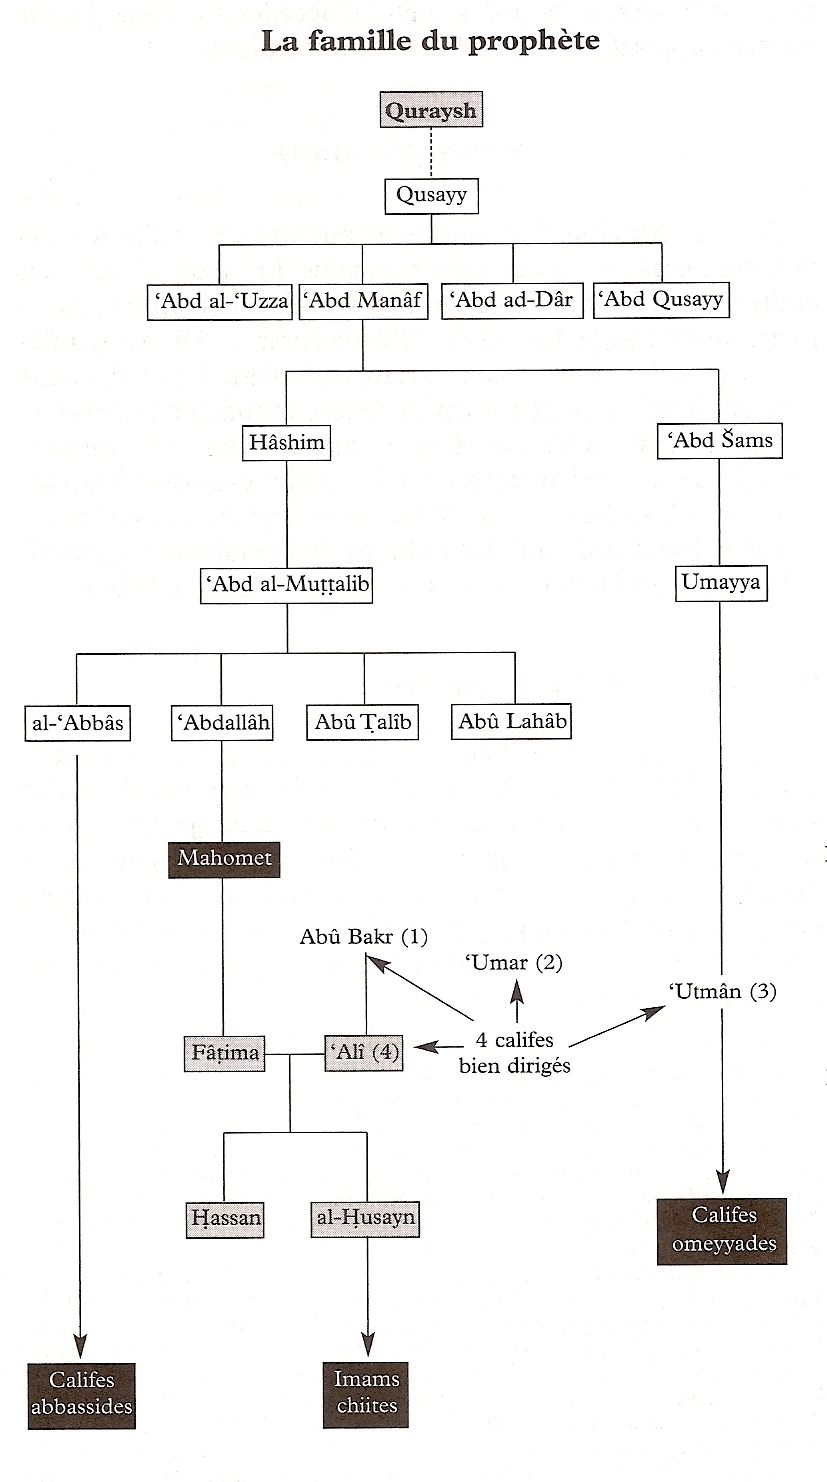
\includegraphics[width=4.31134in,height=7.72685in]{Images/image039.png}

Ce tableau montre bien que les abbassides descendent des ḥāšimites, d'où
vient Muḥammad. Ils sont donc plus proches de sa lignée que les
Omeyyades. En soulignant l'importance du lien familial et du sang, cela
leur octroie une plus grande légitimité.

 
\subsection{Muḥammad dans le ḥadīṯ
 }

Nous accorderons un chapitre au {ḥadīṯ}. Disons d'emblée que le
ḥadīṯ (la collection de ḥadīṯ-s s'appelle {Sunna}) rend compte de
la personnalité de Muḥammad mais aussi et surtout de ses goûts~: de ce
qu'il aime, de ce qu'il déteste~: il aime les sucreries, le miel, les
chevaux, les petits enfants, le pain trempé dans du vinaigre\ldots{} il
déteste les perruques, les barbes épaisses, la torture des hommes ou des
animaux domestiques, les hommes voraces, les vêtements violets, le
bavardage sur le bord du chemin, les serpents et les lézards, la poésie,
le fait de maudire, jurer ou harceler.

Comme nous le verrons, toutes ces informations ne sont pas sans
difficulté dans l'appréciation de leur vérité historique.

Le ḥadīṯ donne à entendre les ordres de Muḥammad, ses recommandations,
ses décisions, son discernement devant des situations particulières.
Ainsi, si le Coran invite au \textbf{ǧihād}, le ḥadīṯ établit une
\textbf{hiérarchie} avec le devoir d'attention à ses parents.

{«~Un homme vint voir Muḥammad avec l'intention de partir pour le
ǧihād. Muḥammad lui demanda~: est-ce que tes parents sont vivants ? Oui,
répondit-il. Alors va et accomplit le ǧihād en prenant soin d'eux, dit
Muḥammad~».}

La base de la biographie de Muḥammad s'appuie sur les textes rédigés de
manière organisée par Ibn Isḥāq. C'est le genre littéraire narratif que
l'on appelle Sīra.


\subsection{Muḥammad dans la Sīra
}

La Sīra n'est pas le ḥadīṯ~: elle est un genre littéraire particulier.
Elle est fixée par quelques auteurs dont Ibn Iṣḥāq, Ibn Hišām, al-Wāqidī
(m. 822), Ibn Sa`d (m. 845), al-Ṭabarī (m. 923). Contrairement au ḥadīṯ,
ce sont des écrivains ; ils ne sont pas des transmetteurs. Ils écrivent
une vie de Muḥammad, ils l'organisent donc. Certes, les chaînes de
transmission ({isnād}) se retrouvent aussi dans la Sīra, mais elle
est un récit structuré autour d'une histoire. Le ḥadīṯ met en avant
Muḥammad comme enseignant~; la Sirā apporte la dimension historique de
Muḥammad. La Sīra inclut les expéditions militaires. Les auteurs des
Sīra écrivent dans des contextes politiques et idéologiques situés entre
100 et 250 de l'Hégire. Les conquêtes ont eu lieu, le šīʿisme s'est
séparé du sunnisme, des controverses avec les chrétiens ou les juifs ont
été engagées. Ces éléments se retrouvent bien sûr en arrière fond de la
Sīra.

Par ailleurs, l'histoire a une vocation éducative. Un fait peut fort
bien être douteux mais s'il a une valeur morale, éthique, l'écrivain la
retient, son travail n'est pas d'abord la critique, mais aussi
l'édification de la communauté.

Si chaque Sīra a son expression littéraire, on peut néanmoins distinguer
sept séquences qui témoignent d'un certain ordre chronologique.


\paragraph{Les sept séquences
chronologiques}

1/ la généalogie de Muḥammad, son enfance, les signes miraculeux qui
annoncent une destinée prophétique~: il s'agit de rattacher Muḥammad à
l'origine de l'humanité, de tout temps, il est prophète. Mais aussi de
montrer qu'avant la révélation coranique des signes extérieurs reconnus
par les communautés juives et chrétiennes indiquaient la mission que
Dieu lui avait destinée.

2/ le jeune Muḥammad jusqu'à son mariage avec Ḫadīǧa.

Un enfant pauvre, orphelin, bref dans une situation d'une grande
précarité. Il est question de ses croyances. Certains récits attestent
qu'il était monothéiste, d'autres qu'il suivait les croyances de sa
tribu. Ce qui est intéressant, c'est qu'en dépit de leur caractère
contrasté, contradictoire, la tradition a gardé ces récits. Il aurait
été plus facile de tout uniformiser. Ce mariage avec Ḫadīǧa alors qu'il
a 25 ans et qu'elle en a 35 ou 40 fait l'objet de plusieurs versions~:
dans certains récits, son oncle l'a marié avec Muḥammad, dans d'autres,
elle a fait boire son père avec la complicité de sa sœur pour obtenir
son accord en vue du mariage. Parfois, les historiens rapportent des
versions différentes et interviennent en disant ce qu'ils considèrent
comme étant la version la plus probable du point de vue historique.

3/ le commencement de la révélation. Il a quarante ans. On dénombre plus
d'une centaine de récits narrant le jour de la révélation, la réaction
de Muḥammad, le partage avec les siens, sa peur de la folie~; il va même
jusqu'à envisager de mettre fin à sa vie.

4/ Sa prédication et sa réception difficile auprès des Mecquois, période
douloureuse qui s'achève avec la mort d'Abū Ṭālib (c'est l'oncle
paternel de Muḥammad qui l'a élevé après la mort de sa mère, avec son
grand père) et de Ḫadīǧa. C'est une période d'épreuves si bien que les
premiers musulmans qui suivent Muḥammad sont considérés comme des héros.
Dans un milieu hostile, où le Prophète est ridiculisé, insulté, ils ont
tenu ferme. C'est dans ce cadre que les noms de ceux qui insultent sont
donnés. Au départ, Muḥammad prêche dans le secret, puis sur des lieux
publics. On voit un homme du nom de `Uqba lui porter un coup sur la
nuque alors qu'il est en prière. Mais la Sīra rend compte aussi de la
justice divine car tous les ennemis de Muḥammad mourront dans d'atroces
maladies, ou de soif, ou au combat~; certains meurent tués par des
animaux sauvages ou capturés, puis tués par Muḥammad lui-même. L'ange
Gabriel n'est pas seulement celui qui transmet la parole mais il prend
part au combat contre Satan. Il est celui qui venge le messager de Dieu.
C'est au cours de cette période que Muḥammad réalise le Voyage nocturne
de La Mecque à Jérusalem. Mais à ce voyage horizontal a aussi succédé un
voyage vertical~: il s'agit des visions du ciel et de l'enfer.

5/~Il s'ensuit la période de l'Hégire à Médine, l'établissement de la
communauté, la mise en place des rituels et des lois, la croissance de
son autorité, les batailles. Cette partie occupe en moyenne 75\% des
Sīra. C'est la période où se constitue une communauté politique, un
proto-état. Dieu est avec Muḥammad et le rend victorieux de toutes les
batailles à l'intérieur de Médine comme à l'extérieur. Des centaines de
personnalités sont convoquées. On ne raconte plus seulement la vie de
Muḥammad mais aussi celle de la première communauté. Le récit des
batailles fait l'objet de longues descriptions. Les anges prennent part
à ces batailles/ Sont données les listes des combattants, des ennemis,
des hypocrites, des morts, des prisonniers. Une attention particulière
est donnée aux dates de chaque évènement. Muḥammad s'affirme toujours
davantage, il présente un visage déterminé, mais aussi une personnalité
capable de pardonner à ses ennemis. Mais on le voit aussi intransigeant,
déterminé, ordonnant l'exécution et la mort de certains de ces ennemis. \sn{Al-Waqīdī, Kitāb al-maġāzī, éd. Marsden Jones,
  London, Oxford University Press, 1966, 1, p. 113-14.}\textsuperscript{.}
\begin{quote}
{«~Le Prophète ordonna à `Asim Ibn Ṯābit de décapiter la tête de
`Uqba Ibn Abī Muʿayt qui avait été capturé dans une bataille par
`Abdullāh Ibn Salama. `}Uqba se mit à protester{~: `Hélas, O
qurayshites, pourquoi moi je devrais mourir parmi ces prisonniers~?} Le
Prophète répondit~: `Parce que tu es un ennemi de Dieu et de son
Prophète'. `Aqba dit~: `Ton pardon est meilleur. Traite-moi comme tu
traites les autres de mon clan. Si tu les tues, tue-moi~; si tu leur
pardonnes, pardonne-moi~; si tu acceptes une rançon d'eux, accepte-la de
moi. O Muḥammad, qui prendra soin de ma petite fille~?' Muḥammad
répondit~: `Va au diable~! O `Asim, plie son cou vers l'avant et
coupe-le'. `Asim trancha sa tête. Le Prophète dit~: `Tu étais le pire
des hommes, Par Dieu, je n'ai jamais rencontré un homme plus mécréant
envers Dieu, son Prophète, son Livre, ni aussi nocif envers son
prophète. Je remercie Dieu qui t'a tué et m'a rendu
satisfaction'~»
\end{quote}


Comme le remarque Tarif Khalidi, c'est la figure de Muḥammad roi qui
émerge dans la Sīra, un homme qui dispose de la vie ou de la mort sur
autrui\sn{Tarif Khalidi, op. cit., p. 89.}\textsuperscript{.}

Ce qu'il y a de frappant dans la Sīra c'est qu'elle est telle une caméra
qui suit Muḥammad dans les moindres lieux où il se rend. On le voit
sourire, rire, mais aussi malheureux lors de la mort de son fils
Ibrahim, de son oncle Hamza, lors de l'accusation de son épouse `Ā'iša
d'adultère, sans compter les actes de désobéissance de ses compagnons.
Muḥammad est Jésus à La Mecque, annonçant un message, mais Moïse à
Médine, organisant une communauté religieuse et politique.

6/ La reconquête de La Mecque~en 630. Muḥammad s'impose comme un chef,
un guide. On voit des délégations de tribus venir lui faire allégeance.
Il est supposé avoir écrit une lettre à l'empereur byzantin, au shah de
Perse\ldots{} Sa mission s'universalise aux quatre coins de la terre.

7/ Enfin, nous avons la dernière phase de sa vie~: sa maladie jusqu'à sa
mort. Récemment, Hela Ouardi, historienne tunisienne, a consacré une
recherche sur les récits évoquant la mort de Muḥammad dans la tradition
musulmane. L'ouvrage a fait pas mal de bruit parce qu'il contredit
l'image d'une communauté unie, endeuillée, par la mort de son
Prophète\sn{Hela Ouardi, Les derniers jours de Muḥammad, Paris,
  Albin Michel, 2015.}. Qui plus est, elle montre que nombreux étaient
ceux qui cherchaient à l'éliminer. Et le Prophète est de plus en plus
méfiant. Alors qu'on lui administre un médicament, il demande aux
personnes présentes de prendre aussi de la potion médicinale. On voit
aussi que son corps est oublié et qu'il n'est pas enterré. La communauté
semble préoccupée d'abord par la question politique~: qui va le
remplacer~? Mais le corps se fait rappeler à lui par son odeur~!

Quelques précisions sur les particularités et les contextes
rédactionnels des premiers auteurs de Sīra.


\paragraph{Les récits d'Ibn
Isḥāq}

La Sīra d'Ibn Iṣḥāq est composée vers 150 / 772. Ces récits sont la base
de toute biographie qui portera sur Muḥammad telle qu'elle s'est
diffusée dans la tradition islamique. Ibn Isḥāq les aurait rédigés,
enseignés ou écrits, à la suite d'une commande du calife abbasside
al-Mansūr (754-775) pour son fils, le prince héritier, al-Mahdī. Nous ne
possédons aujourd'hui que des versions remaniées datant du 9ème siècle,
parfois divergentes. Ce texte est néanmoins fondamental. On y trouve le
nom des compagnons de Muḥammad, celui de ses détracteurs, le récit des
batailles de Badr et des autres (Uḥud, Khandaq\ldots), le texte de la
Constitution de Médine (Ṣaḥīfa) \ldots{} que vous avez pu lire dans le
précédent chapitre.

Retenons qu'il semble que le modèle de cette Sīra soit celui des
Évangiles (au sens large, c'est-à-dire canoniques et apocryphes, en tant
qu'ils apparaissent comme une vie de Jésus. Et de fait, il y est
question de signes célestes (pensez à l'étoile des mages), de l'enfance
de Muḥammad, de miracles, de sa prédication, du succès populaire mais
aussi de l'hostilité des notables (les foules versus les
grands-prêtres)\ldots{}

Parmi les versions remaniées, on trouve celle rédigée par \textbf{Ibn
Hišām} (m. 830)~; elle est la version la plus répandue et l'objet de
nombreux commentaires. C'est celle que je vous ai conseillé d'acquérir.
Revoyez la bibliographie générale. Le livre y figure. Le traducteur est
libanais, c'est~: Wahib Atallah.

Les rectifications ou amendements apportés à la biographie \textbf{d'Ibn
Isḥāq} s'expliquent en raison du caractère contrasté et polémique d'Ibn
Isḥāq. Il serait en effet rentré en conflit avec le gouverneur de Médine
car il serait allé interroger sa femme. Ensuite, il aurait eu un conflit
avec Mālik, éminent représentant de la tradition musulmane, en estimant
que certaines de ses informations devaient être relativisées. Mālik est
un des fondateurs des quatre grandes écoles de jurisprudence musulmane
(fiqh). Nous en avons déjà rencontré deux~dans le premier chapitre~:
l'Imām al-Šāfi`ī et Abū Ḥanīfa. Il reste donc un quatrième nom à
découvrir. Patience. Cela viendra\ldots{} plus vite que vous ne pensez.
Mālik alla parfois à le traiter d'imposteur. De même, on lui reprocha
ses tendances ši`ites, ou de collecter des informations à partir des
juifs et des chrétiens. On lui reprocha aussi d'avoir inséré des vers
dans sa biographie et d'avoir fait œuvre de faussaire~! Bref, son œuvre
ne plut pas à tout le monde. D'ailleurs, il faut bien voir que la Sīra
ne jouit pas du même statut que le Coran ou la Sunna (cette dernière
rassemble les paroles du Prophète Muḥammad).~Nous avons rencontré ce mot
dans le premier chapitre à propos de la définition de l'islam.


\paragraph{Ibn Hišām (cAbd
al~Malik)}

On l'appelle \textbf{Ibn Hišām} et retenir ce nom suffira, mais son nom
complet est plus précis: c'est Abū Muḥammad cAbd al~Malik b. Hišām b.
Ayyūb al~Ḥimyarī Ǧamal al~Dīn (m. 218/833 ou 213/828. Le b. est pour Ibn
qui signifie fils de). C'est un généalogiste et grammairien arabe né à
Bassora (Baṣra, en Irak).

\begin{marginfigure}
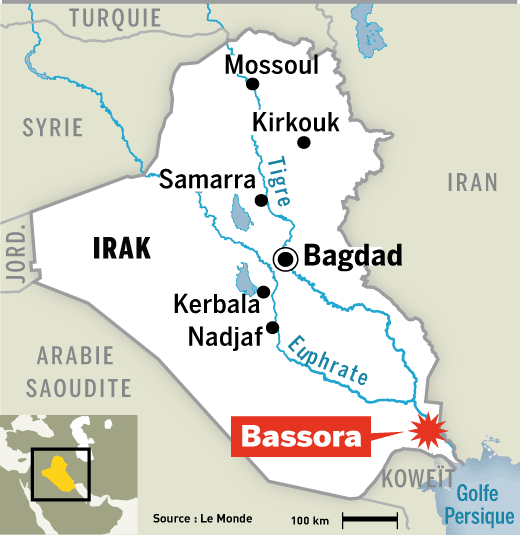
\includegraphics[width=1.42033in,height=1.46065in]{Images/image040.png}
\end{marginfigure}
 

Sa Sīra, comme celle d'Ibn Isḥāq, n'est pas à proprement parler un
document d'histoire. Elle est tributaire de la manière de raconter
propre à l'époque, du style utilisé pour écrire et transmettre. Ce récit
est donc dépendant du contexte culturel, mais aussi des conflits de
personnes ou des tendances qui sont déjà bien nettes, ce qui est
fondamental pour en avoir une juste appréciation.


\paragraph{Et les autres Sīra-s de l'époque
classique}

Dans un souci de précision, je vous donne le nom d'autres auteurs
importants de Sīra. Mais ils sont moins cités que les deux précédents.
Si vous retenez les deux premiers, ce sera donc très bien.
Contentez-vous de savoir qu'ils ne sont pas les seuls à être mobilisés
comme références biographiques.

- Al~Wāqidī (m.~207/823) est un juriste et historien arabe ayant vécu à
l'âge d'or des Abbasides, dont les travaux sur l'époque de Muḥammad
n'ont cessé de faire autorité chez les savants musulmans. Son œuvre se
trouve dans le Kitāb al~Maġāzī ou «~Livre des expéditions militaires (de
Muḥammad)~»\sn{The Kitab al-Maghazi of al-Waqidi, éd. Marsden
  Jones, 3 vol., Oxford University Press, London 1966, réimpr.
  Mu'assasat al-Aclamī li-l-maṭbūcāt, Beyrouth, 1989.}. Il y dresse
l'inventaire chronologique des batailles.

- Muḥammad Ibn Sacd (m.~230/845) est un traditionniste irakien (né à
Bassorah) donc comme Ibn Hishām et mawlā des Hachimides) qui mena ses
activités de transmetteur à l'âge d'or des Abbasides et laissa un
matériel historique apprécié des générations ultérieures. Il a laissé,
parmi d'autres écrits, le «~Livre des générations »\sn{Kitāb
  al-ṭabaqāt al~kabīr, éd. Eduard Sachau et al, 8 vol. (1904-1917) +
  indices E.J. Brill, Leiden, 1928. Il existe une traduction anglaise
  partielle~par Aisha Bewley, The Men of Madina, 2 vol., Ta-Ha
  Publishers, Londres 1997.} (ou «~Livres des classes~»). C'est le genre
littéraire fameux qu'on appelle en arabe les {Tabaqāt}  Cela lui valut la célébrité en fournissant des informations
sur plus de quatre mille personnes ayant, du début de l'islam à l'époque
de l'auteur, transmis des hadīṯs. Ce terme a déjà été vu quand nous
avons donné la définition de l'islam. Cet ouvrage comporte
principalement, outre une biographie de Muḥammad, des notices détaillées
sur les Compagnons ainsi que des données plus brèves sur les personnes
des périodes suivantes.
\begin{Def}[Tabaqāt -classement par génération]
 Certains dictionnaires biographiques rangent les biographies
  par ṭabaqāt c'est-à-dire, «~strates, classes ou générations~»~;
  d'autres par ordre alphabétique. 
 

\end{Def}
Quelques dictionnaires concernent
  uniquement les personnages ayant vécu ou séjourné dans une ville
  déterminée~: ils portent alors généralement le titre trompeur {Tārīḫ} ou
  «~Histoire~» de telle ville, mais ne contiennent en fait que des
  notices individuelles auxquelles s'ajoute une introduction
  topographique sur la ville en question, introduction qui peut être,
  elle aussi, de grand intérêt. \sn{Cf. Hafsi, Ibrahim, «~Recherches sur le
  genre `Ṭabaqāt' dans la littérature arabe~», Arabica 23 (1976),
  227~249.} 
\FloatBarrier
- Enfin, je renvoie à la Sīra d'al~\textbf{Ṭabarī} (m. 310/923), fameux
savant, historien et exégète, originaire du Tabaristan (aujourd'hui
Mazandaran, province de l'actuelle république d'Iran), qui illustra
l'âge d'or des Abbasides et qui demeure une source indispensable à toute
connaissance des événements survenus aux trois premiers siècles de
l'islam. Il créa sa propre école juridique qui ne devait avoir qu'une
existence éphémère. En théologie, il polémiqua \textbf{contre les
interprétations anthropomorphistes} des hanbalites. Et voilà la
4\textsuperscript{ème} école juridique. Donc si je récapitule~:
\textbf{hanafite, shafi`ite, malikite et hanbalite}. Son œuvre écrite
comprend d'abord un {tafsīr}, c'est-à-dire un commentaire
coranique.


\paragraph{{tafsīr}}
\begin{Def}[tafsīr]

commentaire
coranique

\end{Def}

C'est un mot clef, il reviendra souvent, forcément, surtout quand nous
aborderons le cours sur le Coran. Elle comprend aussi une histoire
universelle qui commence avec la création du monde et qui continue
ensuite sa relation des faits jusqu'à l'année 915 en choisissant la
forme d'annales à partir du début de l'ère musulmane. Cette relation
monumentale, qui présente d'un même épisode des versions diverses
reposant, soit sur des informations orales, soit sur des ouvrages
antérieurs, sans porter pour autant de jugement, reste en apparence
aussi objective que possible. En fait elle privilégie certains
événements et elle se montre parfois tendancieuse, au moins par ses
omissions. Il ignore pratiquement le califat omeyyade et l'Occident
musulman.

\paragraph{Muḥammad, modèle du bel agir pour les
musulmans}

Au cours des premiers siècles se développe sous le règne des abbassides
un genre littéraire appelé {\textbf{adab}} et qui dessine, selon
l'expression de Jean-Claude Vadet, l'esprit courtois du monde
arabo-musulman\sn{Jean-Claude Vadet, L'esprit courtois en Orient
  dans les cinq premiers siècles de l'Hégire, Editions Maisonneuve et
  Larose, 1968.}. Il s'agit d'une littérature attachée à circonscrire
l'éthique de l'homme de cour cultivé. Cette littérature englobe à la
fois les rasā'il (épîtres) et les nasā'ih (conseils aux princes).
{L'adab} désigne ainsi l'ensemble des valeurs que le gentilhomme
musulman, l'adīb, doit acquérir.

L'adab occupe une place fondamentale dans la littérature
arabo-musulmane. C'est là que l'on trouve les informations relatives à
la manière de se comporter envers les non musulmans~; tel des essais,
l'adab mentionne des questions éthiques, politiques, sociétales. Il
regroupe aussi des anthologies. Un des célèbres auteurs de adab est
al-Ǧāhiẓ (m. 868).

Dans le cadre de cette littérature, Muḥammad est présenté comme un
enseignant d'adab. Il est l'archétype de l'adīb. On voit ainsi décliner
les vertus de l'humilité, de la sincérité, de la générosité, illustrées
par l'enseignement de Muḥammad.


\paragraph{La canonisation de Muḥammad~: la
réécriture de la Sīra
}

Nous avons vu que dans les premières biographies, le portrait de
Muḥammad pouvait être contrasté et les épisodes rapportés pouvaient même
être contradictoires. L'écrivain intervenait, mais n'effaçait rien des
éléments biographiques dont il disposait. À la suite de l'adab qui met
en lumière le caractère moral de Muḥammad en vue de l'imiter, on assiste
à l'écriture de nouvelles Sīra~; elles sont d'un genre nouveau que l'on
pourrait appeler hagiographique~: le portrait de Muḥammad est
sacralisé~si bien que, du modèle à imiter, Muḥammad devient lui-même
inimitable. On a un exemple de ces Sirā avec l'andalousien al-Qāḍī ʿIyāḍ
(m. 1149) qui dans son célèbre ouvrage Kitāb \textbf{Al-šifā'} bi taʿrīf
ḥuqūq al-Muṣṭafā, (Le \textbf{livre de la guérison} par la
reconnaissance des droits de l'Élu) fait ressortir les qualités
exceptionnelles et l'infaillibilité de Muḥammad faisant de son savoir
une source sûre. Livre très populaire si bien qu'on dit que «~si l'on
trouve dans une maison le al-Šifā', cette maison ne connaîtra aucune
souffrance et si une personne malade le récite, elle retrouve la
santé~». Muḥammad apparaît comme totalement dépourvu du moindre péché,
qu'il s'agisse d'un péché majeur (kabā'ir) ou mineur (saġā'ir). Il a été
préservé de la moindre faute depuis sa naissance. Il est immaculé.

Dans cette perspective, la biographie va rejeter ou rendre compte de
tous les épisodes qui pourraient ternir l'image de Muḥammad~: ainsi,
l'épisode des versets sataniques est considéré comme absolument
inacceptable~; il est une forgerie pour nuire au Prophète de l'islam. Le
fait qu'il épousa Zaynab, la femme de son fils adoptif, ce qui
contrevient à la loi de la filiation puisque cela constituait un
inceste, est cependant expliqué par le Coran lui-même~(S. 33, 36-40).
Muḥammad n'a fait donc que répondre à un commandement de Dieu, et non à
un désir de la chair.

Mais la question qui se pose est la suivante~: pourquoi assiste-t-on à
ce processus de canonisation de Muḥammad~? de réécriture de la Sīra~?

Le xiie siècle est celui de polémiques sur l'articulation entre la
raison et la révélation, sur le statut de la philosophie et de la
prophétie. Dans ses relations avec les non musulmans, l'élite de la
communauté musulmane doit répondre à de nombreuses accusations à charge
contre le Prophète Muḥammad -- nous en avons vu quelques exemples. La
défense de la prophétie se réalise à deux niveaux~: d'une part, celui de
la tradition où il s'agit de rapporter et de fonder selon la
méthodologie propre des sciences du ḥadīṯ la véracité des miracles qui
sont racontés -- c'est la ligne d'Ibn Qutayba~; et d'autre part,
d'établir des raisons pour justifier la prophétie -- c'est la ligne
d'al-Ǧāhiẓ.

Dans les polémiques avec les chrétiens ou les juifs, certains auteurs
vont fonder à partir de la Bible les preuves de la prophétie de
Muḥammad.


\paragraph{{Les biographies contemporaines de Muḥammad }}

À partir du XIXème siècle, on assiste dans le monde musulman à
l'écriture de nouvelles Sirā~: elles sont des défenses dans un contexte
de publication de la part des orientalistes qui viennent jeter quelques
ombres sur la réputation morale de Muhammad. Comme nous l'avons vu, le
monde occidental et chrétien n'en est pas à ses premières diatribes et
tableaux obscurs, mais ces accusations étaient jusqu'alors souvent
ignorées du monde musulman dans son ensemble et seules les élites
prenaient part aux polémiques. Les travaux des orientalistes dans un
contexte de colonisation donnent une plus grande audience à ces
critiques. C'est d'abord en Inde que l'on trouve ces réactions. Un des
exemples de ces biographies apologétiques est celle écrite par
l'égyptien Muḥammad Ḥusayn Haykal (m. 1956), Ḥayat Muḥammad.

Mais d'un autre côté, prenant au sérieux la critique des orientalistes
du XIXème, des auteurs appellent à revisiter l'histoire de la Sīra. Un
de ces auteurs est notamment l'égyptien Ḥusayn Aḥmad Amīn (m. 2014) dans
son ouvrage {Dalīl al-muslim al-ḥazīn fī muqtaḍá al-sulūk fī
al-qarn al-ʿišrīn} \textit{Le Guide du musulman triste quant à la bonne
conduite pour le vingtième siècle} -- remarquez que le titre un peu
pompeux veut imiter les titres de l'ancien temps\ldots{} et est
ironique~!
\sn{On trouve une traduction française de l'ouvrage~:
  Hussein Amin, Le livre du musulman désemparé. Pour entrer dans le
  troisième millénaire, Paris, La Découverte, 1992. En ligne, l'article suivant~d'où est extrait la dernière
  citation : Hussein Amin, «~La biographie muhammadienne entre Orient et
  Occident~», Égypte/Monde arabe,
  \url{https://ema.revues.org/473}{Première série, 9~\textbar{} 1992},
\url{http://ema.revues.org/1232~; DOI~: 10.4000/ema.1232}} 

Dans le chapitre
2\textsuperscript{ème}, il souligne l'objectivité des premières Sīra qui
se sont attachées à rendre compte des moindres détails, quels qu'ils
soient, et même s'ils étaient contradictoires. On y voit un Muḥammad
fait de chair et de sang, un simple être humain, mais qui a connu une
inspiration divine. Mais Amīn remarque que le temps passant, la Sīra a
dévié et l'on a voulu élever au même rang Muḥammad que celui des grandes
figures religieuses en en faisant un superhéros. Dans la biographie
d'Amīr ʿAlī, {Spirit of Islam}, il s'agit de montrer combien
l'islam et la personne de Muḥammad est en parfaite adéquation avec le
standard de la modernité européenne. Ainsi, on va chercher à montrer
{«~comment l'islam a élevé le statut de la femme, comment il a
atténué la sévérité envers l'esclavage, comment il a promu la recherche
du savoir, construit des hôpitaux, comment il a combattu la
discrimination raciale et établi les bases de la justice sociale~}»
{[}souvenez-vous la définition de l'islam de Si Hamza Boubakeur à partir
des termes de liberté, égalité, fraternité{]}. Pour lui, le problème est
celui d'une congruence entre l'attachement pieux à Muḥammad propre aux
premières Sīra et l'hagiographie des Sīra ultérieures. Il s'en est suivi
une attitude où l'on accuse de diffamation ou de calomnie celui qui
vient à critiquer le portrait porté par la tradition de Muḥammad.

Mais alors quelle vie de Muḥammad, quelle Sīra conviendrait-il désormais
d'écrire au sein de monde musulman~? Quelle Sīra pour le XXème siècle~?
Amīn écrit~:

«~L'heure est venue pour les musulmans d'écrire une nouvelle sîra. Une
biographie sans excuse, sans honte ni apologie. Une biographie qui ne
taise ni n'invente rien, ce qui serait contraire à la vérité, mais aussi
qui ne se contente pas de rapporter les faits, ce qui serait contraire à
l'art. Une biographie qui n'omette pas «~ce qui pourrait blesser
certains~», qui n'impose de tutelle à personne. Une biographie qui fasse
revivre dans son intégralité un moment de l'histoire, reconstruise ses
normes et ses valeurs, son milieu, ses traditions et ses coutumes, pour
replacer clairement dans leur contexte la personnalité et l'œuvre du
Prophète. Une biographie qui prenne vis-à-vis de l'histoire, un point de
vue authentiquement religieux, rédigée dans un bel arabe par un musulman
courageux, sans complexe, fier de sa religion, sûr de sa foi en son
Prophète. La biographie qu'écriraient un Wāqidī, un Ṭabarī, s'ils
vivaient aujourd'hui~».


\paragraph{Conclusion~: entre imitatio Muḥammadi et imitatio
Christi}

Il existe dans le christianisme une spiritualité de la {sequela
Christi}, souvent associée à l'imitatio Christi. À noter que les
chrétiens ne focalisent pas leur regard sur le Christ tel qu'il vivait
il y a deux mille ans, mais sur le Christ en Gloire, mort et ressuscité,
qui se trouve non derrière eux, mais toujours devant eux. L'Évangile et
la vie de Jésus ne sauraient définir un mode de vie à reproduire, des
actions à réitérer, dans la mesure où ces récits historiques sont
appelés à être lus et regardés à la lumière de Pâque dans le cadre d'une
théologie de l'Esprit Saint qui renouvelle toutes choses. Ce qu'il
s'agit d'imiter c'est la Pâque du Christ, le passage à une vie nouvelle,
la capacité d'atteindre et de vivre d'ores et déjà quelque chose de la
résurrection. Et cette transformation, cette conversion se réalise par
la crucifixion du moi égoïste et conduit à l'identification du chrétien
avec le Christ~:
\begin{quote}
    
«~J'ai été crucifié avec le Christ, et si je vis, ce
n'est plus moi qui vis, c'est le Christ qui vit en moi~» 
\end{quote} 
écrit saint
Paul aux Galates (Gal. 2, 20).

\begin{Synthesis}

En islam, l'imitatio Muhammadi est d'un autre ordre. Le Prophète de
l'islam est la mise en œuvre concrète du Coran.
\end{Synthesis}

Il est le témoin de la
possibilité de suivre les commandements divins, il est l'herméneute par
sa vie de ce qu'il faut suivre pour être fidèle à la volonté divine, il
est le beau modèle (Coran 33, 21). On trouvera certes dans la tradition
musulmane des exemples d'enseignements soufis dont la perspective
mystique reflète et approche l'enseignement chrétien à l'exemple
d'al-Bistami (m. 874), mais d'une manière générale, l'activité et les
actions du prophète restent normatives. Quand il s'agit de vertus
morales, et de qualités sociales telles la compassion et la générosité,
l'imitation de Muḥammad est source d'une fructueuse émulation.
\begin{Synthesis}

{Quand il s'agit de légitimer la violence par les armes dans la
lutte contre l'injustice, l'oppression ou l'infidélité, loin d'être
écartée, la violence est légitimée. Aux yeux d'un occidental, cette
violence est hautement problématique et constitue le défi majeur de
l'islam contemporain.}

\end{Synthesis}

\paragraph{Annexe. Éléments de biographie selon la Sīra d'Ibn
Hišām}

Après avoir vu les sources de la Sīra du Prophète de l'islam, nous
allons entrer dans les textes en ouvrant notamment la Sīra d'Ibn Hišam.
Le choix ici est purement arbitraire. Il a cependant pour but de mettre
en lumière des questions d'inter-religiosité, mais aussi
d'intertextualité~: autrement dit, dans quelle mesure la Sīrā éclaire la
question `Muḥammad et les autres religions', comment le texte même de la
Sīra se comprend en lien avec d'autres textes des traditions religieuses
non islamiques~? Pour autant, je suivrai la trame de sa vie~: son
enfance, sa situation familiale, son mariage, le début de la révélation
à La Mecque alors qu'il a quarante ans, l'acceptation puis le rejet des
Mecquois, la fuite à Médine, c'est-à-dire l'Hégire, la mise en forme
d'une législation, les batailles, le retour triomphal à La Mecque.
L'Hégire est la grande date dans l'histoire de l'islam, c'est l'an 1 du
calendrier dit `hégirien'. Cette fuite, alors qu'il est persécuté par
les siens, s'inscrit dans la grande tradition des prophètes bibliques
dans le désert. Elle rappelle la traversée dans le désert d'Agar, la
servante d'Abraham. Dans le désert, Dieu intervient et protège la jeune
communauté musulmane, à l'exemple de l'épisode de l'araignée~: alors que
ses membres se sont cachés dans une grotte, les Mecquois les
recherchent. Ils aperçoivent la grotte, s'approchent, mais renoncent à y
entrer car une araignée y a tissé sa toile. Ils en déduisent qu'ils ne
peuvent s'y être cachés. Voici la trame mais il faut savoir que lors du
Forum islamo-catholique de Lyon en novembre 2014, un imam disait à ses
collègues que «~s'il fallait écrire sur une feuille A4 la vie de
Muḥammad telle qu'elle nous a été enseignée, telle que nous
l'enseignons, tous nous consacrerions les ¾ de la page à mentionner les
récits militaires~». Et en disant cela, pour lui, c'était un problème.


\paragraph{La généalogie
}

Muḥammad était le fils de `Abd Allāh, b. `Abd al-Muṭṭalib, b. Hāšim, b.
`Abd Manāf, b. Quṣayy (\ldots) b. Ismā`īl, b. Ibrāhīm, b. Tāriḥ (\ldots)
b. Nūḥ (Noé) (\ldots) b. Adam.

Si je compte le nombre de parents, il y en a 40\ldots{} comme pour la
Généalogie du Christ de Matthieu.


\paragraph{{Une naissance attendue
}{Une naissance attendue }}

\mn{La naissance de l'Envoyé de Dieu (Sīra, I 155-160)}
\begin{quotation}
    

Les gens disent (Dieu seul sait si c'est vrai) qu'Âmina, la mère du
Prophète, racontait que lorsqu'elle était enceinte, elle eut en songe la
visite d'un homme qui lui dit~: «~Tu portes dans ton sein le seigneur de
cette nation~; dès que tu auras accouché, tu mettras l'enfant sous la
protection de Dieu, l'Unique, à l'abri de la méchanceté des envieux. Tu
l'appelleras Muhammad.~» Âmina racontait aussi que lorsqu'elle fut
enceinte de Muhammad, elle vit sortir d'elle une lumière qui illumina
devant elle les châteaux de Bosra en Syrie.

Outre les raisons qui avaient porté Halîma, la mère nourricière du
Prophète, à rendre l'enfant à sa mère Âmina, raisons qu'elle venait de
lui avouer, il en était une qu'elle avait réussie à garder secrète,
c'est qu'un groupe d'Abyssins (Éthiopiens) chrétiens avaient vu l'enfant
lorsque Halîma le ramenait à la Mecque après son sevrage. Les Abyssins
avaient observé l'enfant, l'avaient tourné et retourné dans tous les
sens, avaient interrogé Halîma à son sujet et lui avaient dit~: «~Nous
allons prendre ce garçon chez nous, pour notre roi\sn{Il s'agit du
  Négus, roi chrétien d'Abyssinie, l'actuelle Éthiopie.}. C'est un
garçon qui a un grand destin, nous le savons.~» Halîma eut beaucoup de
mal à leur échapper.

Bien des années plus tard, quelques compagnons dirent au Prophète~:

- Envoyé de Dieu, parle-nous un peu de toi.

- Je suis, leur dit-il, la vocation de mon père Abraham, la bonne
nouvelle de mon frère Jésus. Lorsqu'elle fut enceinte de moi, ma mère
vit sortir d'elle une lumière qui illumina pour elle les châteaux de
Syrie. J'ai été placé en nourrice chez les Banû Sa'd. Tandis qu'un jour
avec mon frère de lait nous gardions quelques agneaux derrière les
maisons, soudain, je vis deux hommes habillés de blanc qui portaient une
cuvette en or pleine de neige. Ils se saisirent de moi, m'ouvrirent le
ventre et sortirent de mon cœur un caillot de sang noir, qu'ils
jetèrent. Puis ils lavèrent et purifièrent mon cœur et mon ventre avec
cette neige. Enfin, l'un des hommes en blanc dit à son compagnon~:
«~Mets-le en balance contre dix hommes de sa nation.~» Il me pesa et le
plateau de la balance pencha de mon côté. «~Mets-le en balance contre
cent hommes de sa nation, ajouta-t-il.~»~ Il me pesa et je l'emportais
encore. «~Mets-le en balance contre mille hommes de sa nation,
poursuivit-il.~» Il me pesa et je l'emportais toujours. «~Arrêtons,
dit-il. Si on le mettait en balance contre toute sa nation, il
l'emporterait encore.~»

Le Prophète disait~: «~Il n'y a pas eu de prophète qui n'ait été
berger.~» On lui demanda~:

- Et toi, Envoyé de Dieu~?

- Moi aussi j'ai gardé des moutons.

Le Prophète disait aussi à ses compagnons~: «~je suis le plus arabe
parmi vous. Je suis issu des Quraych et j'ai été en nourrice chez les
Banû Sa'd.~»
\end{quotation}

La Sīra réinvestit l'enfance de Muḥammad pour lui donner une dimension
prophétique. On est dans ce que l'on appelle un topos \sn{Topos, topique (ou lieu commun) Un topos est un sujet littéraire qui revient souvent jusqu'à constituer un thème récurrent et attendu dans la littérature} littéraire.


\paragraph{L'enfance du Prophète (Sīra, I,
179-187)}
    
\begin{quotation}
Après la mort de son grand-père, l'enfant fut élevé par son oncle Abû
Tâlib, sur la recommandation, dit-on, de `Abd al-Muttalib Abdallah, père
de Muhammad, et Abû Tâlib étaient en effet deux frères du même père et
de la même mère.

Abû Tâlib préparait le départ d'une caravane de commerçants pour la
Syrie. Quand tout fut prêt et que les hommes furent sur le point de
partir, Muhammad se jeta au cou de son oncle. Abû Tâlib, tout ému,
s'écria~: «~Je vais l'emmener avec moi en Syrie. Nous ne nous quitterons
jamais.~» Il le prit donc dans sa caravane. Ils atteignirent Bosra de
Syrie. Là, dans un monastère, vivait un moine chrétien appelé Bahîra,
qui puisait sa science du christianisme dans un livre conservé au
couvent et transmis de génération en génération. Souvent la caravane
faisait halte près du monastère sans que Bahîra l'invite ou l'aborde.
Cette année-là, Bahîra fit dire à la caravane des Quraych qu'il avait
préparé un grand repas à leur intention et qu'il aimerait que tous y
participent, grands et petits, hommes libres et esclaves. L'un des
Quraych dit à Bahîra~:

- Tu dois sûrement avoir une arrière-pensée aujourd'hui. Nous sommes
passés souvent par là, sans que tu nous invites. Que t'arrive-t-il
aujourd'hui~?

- C'est vrai~; je ne vous invitais pas. Mais vous êtes toujours mes
hôtes et j'ai souhaité, pour vous honorer, que vous soyez tous
aujourd'hui mes invités à ce repas.

Ils répondirent tous à l'invitation, sauf Muhammad qu'on avait laissé
près de la caravane, sous un arbre, en raison de son jeune âge. Lorsque
Bahîra fit le tour de ses hôtes, il ne trouva pas Muhammad parmi eux.

- Je vous avais bien demandé, leur reprocha-t-il, qu'à ce repas personne
ne fût absent.

- Oui, Bahîra, personne n'est absent, sauf un jeune garçon qui est resté
près de la caravane.

- Je l'invite quand même à prendre ce repas avec vous.

Un homme des Quraych alla prendre Muhammad dans ses bras et le fit
asseoir avec les hommes. Bahîra observait le jeune garçon et scrutait
chaque partie de son corps pour la comparer avec ce qu'il en avait lu
dans les livres. Le repas terminé, les hommes se dispersèrent. Bahîra
s'approcha alors de Muhammad~:

- Je t'adjure, lui dit-il, de répondre aux questions que je vais te
poser.

- Pose-moi toutes les questions que tu veux.

Bahîra lui posa toutes sortes de questions sur son sommeil, sur son
comportement et sur ses relations. Muhammad y répondit et ses réponses
correspondaient aux lectures de Bahîra. Puis le moine découvrit le dos
du garçon et il y reconnut entre les épaules le sceau de la prophétie, à
l'endroit même signalé dans les livres. Ce sceau était comme la marque
d'une ventouse sur la peau.

Bahîra s'adressa à l'oncle de Muhammad et lui dit~: Maintenant, tu dis
la vérité. Ramène cet enfant dans son pays et protège-le des juifs. En
effet, s'ils le voient et s'ils savent ce que je sais de lui, ils vont
certainement lui vouloir du mal. En vérité, ton neveu aura un grand
destin. Ramène-le au plus vite chez lui.

Devenu jeune homme, il était, dans sa tribu, le plus courageux, le plus
doux de caractère le plus noble de naissance, le meilleur voisin, le
plus sage, le plus sincère, le plus fidèle. A tel point que les gens
l'appelaient le Fidèle (al-Amin). Dieu avait en effet réuni en lui
toutes les qualités.

Le nom de ce moine Bahīra est un classique. Il s'agit d'inscrire la
naissance de Muḥammad au sein d'une attente prophétique (messianique
dans le cas du Christ). Il se retrouve dans la littérature chrétienne
sous le nom de Serge ou de Nestor. Il est considéré comme hérétique.

Ce moine gardait précieusement les Écritures~: autrement dit, elles
n'ont pas été altérées, falsifiées, ce qui est un gage d'authenticité.
\end{quotation}

\paragraph{Ḫadīğa, épouse du Prophète (Sīra,
I,187-192)}
\begin{quotation}
    
Ḫadīğa est un fille de haute lignée, elle a épousé plusieurs hommes et
est dotée d'une fortune personnelle importante.

À l'âge de vingt-cinq ans, Muḥammad épousa Khadîja bint Khuwaylid.
C'était une noble et riche commerçante, qui engageait des hommes pour
son commerce et les intéressait aux bénéfices.

Hamza, un oncle de Muhammad, l'emmena chez Khuwaylid ibn Asad, père de
Khadîja, et demanda pour son neveu la main de sa fille.

Khadîja donna au Prophète tous ses enfants, sauf Ibrâhîm~: al-Qâsim,
at-Tâhir et at-Tayyib. On appelait Muhammad Abû-I-Qâsim, (kunya), du nom
de son fils aîné al-Qâsim. Ces trois garçons moururent avant la mission
du Prophète. Khadîja lui donna comme filles Ruqayya puis Zaynab puis Umm
Kulthûm et enfin Fâtima. Toutes connurent l'islam, s'y convertirent et
émigrèrent à Médine avec leur père. Quant à Ibrâhîm, sa mère était Mâria
l'Égyptienne, concubine du Prophète qui lui avait été offerte par
Muqawqis, le roi d'Égypte.

Tabarī raconte dans les Chroniques que le Père de Khadija ne voulut pas
donner la main de sa fille. Celle-ci procéda à une ruse~: elle invita
les notables de Qurash, son père et l'oncle de Muḥammad. Le vin coula à
flots, et l'oncle de Muḥammad, Abū Tālib, put faire la demande\ldots{}
le père de Khadija enivré, accepta. Le lendemain, il fut furieux, mais
c'était trop tard.
\end{quotation}


\paragraph{L'annonce de la mission prophétique
}

Quelques hommes des Qurayš portent leur réflexion sur les différentes
religions (Sīra, I, 222-232)
\begin{quotation}
    

Les Quraych étaient réunis, un jour de fête, autour d'une de leurs
idoles qu'ils vénéraient. Ils lui avaient offert des sacrifices, avaient
participé à la cérémonie et à la ronde rituelle autour d'elle. Quatre
d'entre eux, dans une conversation privée, se dirent~: «~Soyons francs
et discrets. Il est clair que notre peuple est dans l'erreur et qu'il a
altéré la religion d'Abraham. Qu'est-ce que cette pierre autour de
laquelle nous faisons des rondes rituelles (tawâf)~? Elle n'entend
rien~; elle ne voit rien~; elle ne fait pas de mal~; elle ne fait pas de
bien~! Trouvons-nous une autre religion.~» Ces quatre hommes étaient
Waraqa ibn Nawfal, `Ubayd Allâh ibn Jahch, `Uthmân ibn al-Huwayrith et
Zayd ibn `Amr. Depuis, ils se dispersèrent à travers le monde, à la
recherche de la religion d'Abraham (Hanîfiyya).

Waraqa ibn Nawfal, le cousin de Khadîja, épouse du Prophète, adopta le
christianisme~: il apprit les Écritures auprès des maîtres et acquit des
connaissances solides dans cette religion.

Quant à `Ubayd Allâh ibn Jahch, un cousin du Prophète, il resta dans
l'équivoque jusqu'à sa conversion à l'islam. Puis il émigra avec les
musulmans en Abyssinie, accompagné de sa femme Umm Habîba, fille d'Abû
Sufyân, qui était elle aussi musulmane. Arrivé en Abyssinie, il quitta
l'islam et embrassa le christianisme. Il mourut chrétien dans ce pays.
Cet homme, devenu chrétien, fréquentait les compagnons du Prophète en
Abyssinie et ne cessait de leur répéter~: «~Nous avons vu la lumière
alors que vous la cherchez encore~!~»~~ Après la mort de `Ubayd Allâh,
le Prophète épousa sa femme Umm Habîba, fille d'Abû Sufyân.

Quant à `Uthmân ibn al-Huwayrith il se rendit chez César, le roi des
Byzantins. Il embrassa le christianisme et acquit une position
importante auprès de lui.

Enfin, Zayd ibn `Amr ibn Nufayl resta en dehors du judaïsme et du
christianisme. Il quitta cependant la religion de son peuple et il
abandonna le paganisme. Il s'abstenait de la viande d'animaux étouffés,
du sang et des victimes sacrifiées au pied des idoles. Il interdisait
d'enterrer vivantes les jeunes filles et déclarait aux Quraych~:
«~j'adore le Dieu d'Abraham.~Je suis le seul parmi vous à pratiquer
encore la religion d'Abraham.~» Puis il ajoutait~: «~Dieu, si je savais
quelle religion tu préfères, je l'adopterais. Mais je ne le sais pas~!~»

Les Quraych le maltraitaient et le persécutaient, de peur qu'il ne jette
le discrédit sur leur religion. Il quitta enfin La Mecque à la recherche
de la religion d'Abraham. Il parcourut tout le pays, interrogeant les
moines et les rabbins. Il parvint enfin en Syrie où il trouva, sur les
hauteurs de Balqâ', un moine qui connaissait bien le christianisme. Zayd
interrogea le moine sur la Hanîfiyya, la religion d'Abraham. «~Tu
recherches une religion à laquelle tu ne trouveras personne aujourd'hui
pour te conduire. Cependant, le temps est proche où un prophète sortira
de ton pays que tu viens de quitter et prêchera la religion d'Abraham.
Rejoins-le, car c'est bien la période prévue pour sa mission.~» Zayd,
qui avait eu quelques notions de judaïsme et de christianisme et n'en
avait retenu aucune, prit sans délai la direction de La Mecque. Mais,
arrivé dans le pays des Lakhm, des brigands se jetèrent sur lui et le
tuèrent. On raconte que son fils Sa'îd ibn Zayd et `Umar ibn al-Khattâb
(le futur calife), qui était son cousin, demandèrent un jour au
Prophète~:

- Pouvons-nous implorer le pardon pour Zayd ibn `Amr~?

- Oui, répondit le Prophète, car il sera ressuscité, tout seul comme
s'il était une nation entière.
\end{quotation}
{Texte essentiel sur la situation religieuse racontée par Ibn
Hisham. Il y est question de la \textbf{hanīfiyya}, la religion primitive, celle
de l'unicité pure. Le Coran la mentionne en disant d'Abraham qu'il
n'était ni juif ni chrétien, mais hanīf et muslim (S.3, 67).}

On voit que la Sīra identifie Waraqa Ibn Nawfal comme chrétien vivant


\paragraph{Qualités de l'Envoyé de Dieu selon l'Evangile (Sīra, I,
232-233)}
\begin{quotation}
    

Ibn Ishâq a dit~: lorsque Jean l'Apôtre voulut faire connaître aux
chrétiens ce qu'avait écrit, sous l'inspiration de Dieu, Jésus fils de
Marie dans l'Évangile, au sujet de l'Envoyé de Dieu, Jean copia les
phrases suivantes~: «~Celui qui me hait hait Dieu. Si je n'avais pas en
leur présence accompli des merveilles que personne d'autre avant moi
n'avait accomplies, ils ne seraient pas coupables. Mais ils abusèrent de
la grâce et crurent qu'ils l'emporteraient sur moi et sur Dieu lui-même.
Il faut cependant que le mot écrit dans la Loi soit accompli~: «~Ils
m'ont haï gratuitement, sans raison.~» Et lorsqu'al-Munhamanna viendra,
celui que Dieu vous enverra de sa part, l'Esprit-Saint, celui qui a
émané de Dieu, il portera témoignage sur moi. Vous aussi vous porterez
témoignage, car vous avez été avec moi. C'est pourquoi je vous ai dit
cela afin que vous n'ayez pas de doute.~» Al-Munhamanna en syriaque veut
dire~: Muhammad, et en grec~:
al-baraqlîtos\sn{Ces explications philologiques sont données par
  Ibn Hichâm lui-même dans le texte de la Sīra. Il s'agit d'une réponse
  aux chrétiens de son époque.}\textsuperscript{.}
\end{quotation}
Dans l'apologétique musulmane, l'annonce de la venue par Jésus du
Paraclet a été compris non comme celle de l'Esprit Saint mais de
Muḥammad. Dans cette optique, les chrétiens ont compris l'annonce de
Jésus en raison d'un truchement linguistique.


\paragraph{Mission de l'Envoyé de Dieu (Sīra,
I,233-239)}
\begin{quotation}
    

Dieu fit aimer la solitude à l'Envoyé de Dieu, de telle sorte qu'il se
plaisait beaucoup à se retirer seul, loin du monde. Il avait l'habitude
tous les ans de faire une retraite d'un mois à Hirâ (à deux lieues de La
Mecque), où il donnait à manger aux pauvres qui le sollicitaient.
C'était une pratique de la Hanîfiyya à laquelle se livraient certains
hommes des Quraych avant l'islam. Au bout d'un mois, il quittait sa
retraite et, avant même de rentrer chez lui, il allait à la Ka\TArabe{ٴ}ba
et accomplissait autour d'elle sept rondes rituelles.

{L'année où Dieu voulut l'honorer et lui attribuer sa mission
prophétique, à l'âge de quarante ans, au mois de ramadân, l'Envoyé de
Dieu sortit pour sa retraite à Hirâ', comme il avait coutume de le
faire. Il était accompagné de sa famille. La nuit même où Dieu lui fit
l'honneur de sa mission, l'ange Gibrîl (Gabriel) vint le voir. L'Envoyé
de Dieu racontait~: tandis que je dormais, Gibrîl se présenta à moi,
tenant un étui en feutre brodé contenant un livre.}

{- Lis, m'ordonna-t-il.}

{- Lire quoi~? demandai-je.}

{Il appliqua alors l'étui sur mon visage, m'empêchant de respirer à
tel point que je crus en mourir. Au risque de m'étouffer, Gibrîl ne
cessa de m'ordonner de lire. Je demandai, excédé~:}

{- Enfin, lire quoi~?}

{- Lis au nom de ton Seigneur qui a créé~!}

{Il a créé l'homme d'un caillot de sang}

{Lis~!...}

{Car ton Seigneur est le Très-Généreux}

{qui a instruit l'homme au moyen du calame}

{et lui a enseigné ce qu'il ignorait. (Coran, 96,1-5.)}

{Je lus. Gibrîl se tut et s'en alla loin de moi. Je me réveillai en
sursaut et ces mots étaient comme gravés dans mon cœur. Je sortis et,
arrivé au milieu de la colline, j'entendis une voix du ciel crier~:
«~Muhammad, tu es l'Envoyé de Dieu et je suis l'ange Gibrîl.~» Je levai
les yeux vers le ciel et je vis Gibrîl sous la forme d'un homme, les
pieds sur l'horizon. Je m'arrêtai et regardai sans bouger. Puis
j'essayai de regarder ailleurs et, à tous les coins de l'horizon, je
n'avais que cette image. Je suis resté ainsi figé sur place, sans
pouvoir avancer ni reculer. Khadîja avait envoyé des hommes à ma
recherche. Ils arrivèrent jusqu'aux hauteurs de La Mecque et s'en
retournèrent auprès d'elle, tandis que j'étais cloué au même endroit.}

{L'image de Gibrîl disparut enfin de ma vue et je revins chez moi.
Je m'assis contre Khadîja, collé à elle. Elle me demanda~:
«~Abû-I-Qâsim¹, où étais-tu~? J'ai envoyé des gens à ta recherche~!~» Je
lui racontai ce que j'avais vu. «~C'est de bon augure, dit-elle. Cousin,
tiens bon~! Tu seras le prophète de cette nation, je le jure par Celui
qui tient ma vie dans sa main.~»}

{Khadîja se leva, s'enveloppa de son manteau et s'en alla chez son
cousin Waraqa ibn Nawfal. Celui-ci avait embrassé le christianisme,
s'était instruit dans les livres et avait beaucoup appris auprès des
gens de la Torah et des Évangiles. Khadîja lui rapporta ce que l'Envoyé
de Dieu lui avait dit avoir vu et avoir entendu. «~Saint, Saint~!
s'exclama-t-il. Khadîja, si tu m'as dit la vérité, Muhammad, je le jure
par Celui qui tient ma vie dans sa main, Muhammad est en train de
recevoir la Grande Loi, celle que reçut Moïse. Il est le prophète de
cette nation. Dis-lui de persévérer.~»}
\end{quotation}
Ce récit est raconté dans de multiples versions (plus d'une centaine).
Dans certaines, le prophète pensa qu'il était fou et voulut se suicider.

Où l'on voit une fois encore le rôle d'un chrétien attestant
l'authenticité de la mission de Muḥammad. En ce sens, la Sīra est
destinée aussi aux chrétiens et a pour but de leur faire prendre
conscience que l'islam qu'ils rejettent -- à l'époque où Ibn Hishām
écrit, fut reconnu par leurs ancêtres.

\vide{la-ruxe9vuxe9lation-de-lislam}{%
\section{La révélation de l'islam}\label{la-ruxe9vuxe9lation-de-lislam}}


\paragraph{Début de la Révélation
(Sīra,I,239-243)}

La révélation du message divin à l'Envoyé de Dieu commença au mois de
ramadân. Dieu a dit~:

{Le Coran a été révélé durant le mois de ramadân.}

{C'est une direction pour les hommes~;}

{une manifestation claire de la direction et de la Loi (Coran,
2,185)}

{Dieu a dit aussi~:}

{Oui nous avons (tiens~! Un dieu unique dit `Nous' dans le coran)
fait descendre}

{durant la Nuit du Décret.}

{Comment pourrais-tu savoir}

{ce qu'est la Nuit du Décret~?}

{La \textbf{Nuit du Décret} est meilleure que mille mois~! (Coran,
97, 1-3).}

Puis la révélation de Dieu à son Envoyé se fit rare pendant un certain
temps et Muhammad en conçut de la peine. C'est alors que Gibrîl lui
apporta la révélation de la sourate de la \textbf{Clarté du jour}, dans
laquelle Dieu lui jure

{-Dieu qui lui a fait l'honneur qu'il sait -- qu'il ne l'a ni
abandonné ni haï~:}

{Par la clarté du jour~!...}

{Par la nuit, quand elle s'étend~!}

{Ton Seigneur ne t'a ni abandonné ni haï~!...}

{Ne t'a-t-il pas trouvé orphelin et il t'a procuré un refuge.}

{Il t'a trouvé errant et il t'a guidé.}

{Il t'a trouvé pauvre et il t'a enrichi\ldots{}}

{Quant aux bienfaits de ton Seigneur, raconte-les. (Coran, 93, 1-3,
6-8,11.)}

L'Envoyé de Dieu se mit donc à raconter les bienfaits que Dieu lui avait
accordés et que, par son intermédiaire, il a accordés aux hommes. Et
c'est ainsi qu'il faisait secrètement part de sa prophétie aux personnes
de sa famille en qui il avait confiance.


\paragraph{Début de l'obligation de la prière (Sīra,
I,243-245)}
\begin{quote}
    

{Lorsque la prière fut imposée à l'Envoyé de Dieu, il était sur les
hauteurs de La Mecque. Gibrîl l'y rejoignit et, d'un coup de talon dans
le flanc de la colline, il fit jaillir une source d'eau. Gibrîl y fit
ses ablutions sous le regard de l'Envoyé de Dieu afin de lui montrer
comment devait se faire le rituel de la purification. L'Envoyé de Dieu
fit alors ses ablutions comme il avait vu Gibrîl les faire. Puis l'Ange
le prit par le bras et lui montra le rituel de la prière et l'Envoyé de
Dieu fit la prière comme il avait vu Gibrîl la faire. Gibrîl s'en alla
et Muhammad rentra chez lui. Il fit ses ablutions en présence de Khadîja
pour lui montrer le rituel de la purification tel qu'il venait de
l'apprendre de Gibrîl. Khadîja en fit de même. Puis Muhammad fit la
prière comme le lui avait appris Gibrîl. Et Khadîja fit de même.}


{Le rituel imposé de la prière était, à l'origine, de deux
génuflexions par prière. Par la suite Dieu le compléta et imposa quatre
génuflexions, lorsque le fidèle était chez lui. Mais, en voyage, la
prière ne devait comporter que deux génuflexions, comme à l'origine.}

{Lorsque l'obligation de la prière fut instituée, Gibrîl se
présenta à l'Envoyé de Dieu à midi, lorsque le soleil était à l'apogée,
et fit la prière avec lui. Puis ils firent la prière ensemble
l'après-midi, au `Açr (au moment où l'ombre de l'homme est égale à sa
taille). Puis ils firent une prière au coucher du soleil, puis une autre
le soir, à la disparition du crépuscule, et une dernière prière le
matin, au lever du jour.}
\end{quote}

\paragraph{Première prédication de l'islam et réaction des Qurayš
(Sīra,I,262-269)}

Les choses se compliquent pour Muḥammad. On cherche à le tuer.
\begin{quote}
    

{Ayant appris qu'Abû Tâlib avait refusé d'abandonner son neveu, les
Quraych lui amenèrent `Umâra ibn al-Walîd~:}

{- Ce jeune homme, lui dirent-ils, est le plus fort et le plus beau
des jeunes gens des Quraych. Prends-le et adopte-le. Il t'appartient. En
échange, livre-nous ton neveu qui a bravé ta religion et la religion de
tes pères et qui a jeté la discorde dans ton peuple. Nous le tuerons,
puisque nous t'en donnons un autre.}

{- Quel triste marché vous me proposez~! Vous me donnez à nourrir
votre fils et je vous donnerais à tuer le mien~! Jamais, au grand
jamais, je n'accepterai~!}

{- Nous avons été équitables avec toi~; mais, c'est clair, tu ne
veux rien entendre.}

{- Non, vous n'êtes pas équitables~! Bien au contraire, vous vous
êtes coalisés contre moi. Faites donc ce qui vous plaît.}

{Les Quraych se concertèrent et chaque tribu décida de faire la
chasse, en son sein, aux adeptes de Muhammad qui avaient embrassé
l'islam, pour les persécuter et les détourner de leur religion. Dieu
protégeait son Envoyé par l'intermédiaire de son oncle Abû Tâlib. Ce
dernier, voyant ce que faisaient les Quraych, alla trouver les Banû
Hâchim et les Banû `Abd al-Muttalib pour les appeler à défendre Muhammad
et à prendre son parti, comme il le faisait lui-même. Ils répondirent
tous à son appel et prirent la défense de l'Envoyé de
Dieu}\sn{On constate ici que la solidarité de clan passe avant
  toute considération religieuse.}{, à l'exception d'Abû
Lahab}
\end{quote}
{Abū Lahab, oncle du Prophète, s'est opposé à Muhammad de
  manière acharnée et irréductible. Il fut l'objet d'une révélation du
  Coran (111,1-3) qui le condamne, lui et sa femme, au feu de l'Enfer.
  Il expliquait, paraît-il, son hostilité au Prophète en se rassurant~:
  «~Si Muhammad est dans l'erreur, j'aurais été fidèle à la foi de mes
  ancêtres. Si Muhammad l'emporte, après tout, il est mon neveu\ldots~»}{,
l'ennemi de Dieu.}


\paragraph{Les Qurayš maltraitent l'Envoyé de Dieu
(Sīra, I, 289-291) et il se défend\ldots{}
}

L'hostilité manifestée à l'Envoyé de Dieu et aux premiers convertis
suscita parmi les Quraych des dissensions nuisibles à leurs intérêts.
Ils soudoyèrent contre lui des vauriens qui lui portaient la
contradiction et le maltraitaient. Mais il continuait, au grand jour, à
critiquer leur religion, à bannir, leurs idoles et à se démarquer de
leur paganisme.

{`Amr ibn al-`Âç (futur conquérant de l'Égypte) racontait~: j'étais
au Sanctuaire un jour que les notables des Quraych y étaient réunis. En
parlant de Muhammad, ils disaient~:~«~cet homme a insulté nos pères et
nos divinités~; il a dénigré notre religion et il a semé la discorde
parmi nous. Nous n'avons jamais souffert pareille chose avant lui.
Tandis qu'ils se plaignaient de la sorte, l'Envoyé de Dieu apparut au
Sanctuaire. Il s'avança, toucha l'angle de la Ka'ba et, en en faisant le
tour, passa devant eux. Ils lui lancèrent une insulte que je n'entendis
pas mais dont je vis l'effet sur le visage de l'Envoyé de Dieu. Au
troisième tour et au dixième tour, ils l'insultèrent encore. L'Envoyé de
Dieu s'arrêta et leur dit~: «~Écoutez-moi, hommes des Quraych, j'apporte
le sabre par lequel vous mourrez égorgés, je le jure par Celui qui tient
ma vie dans sa main~». Cette annonce leur fit peur et les jeta dans la
consternation. Celui qui avait été le plus virulent parmi eux n'avait
plus de mots assez doux pour amadouer Muhammad. Il disait~:
«~Abû-I-Qâsim, ne t'en fais pas, continue ton chemin. Tu n'es point un
ignorant~».}

Déjà à La Mecque, face à la menace d'hommes qui lui veulent du mal,
Muḥammad rétorque et se défend. Il semble que la véhémence virulente de
sa réaction suscita déjà l'inquiétude de ses détracteurs.


\paragraph{`Utba Ibn Rabī'a tente une médiation (Sīra, I,
293-294)}
\begin{quote}
    

{- Si avec tes nouvelles idées, tu veux de l'argent, nous sommes
prêts à t'en collecter jusqu'à ce que tu deviennes le plus riche parmi
nous~; si tu recherches les honneurs, nous t'en comblerons~; si tu veux
le pouvoir, nous te proclamerons notre chef. Et, si cet être qui te
hante et t'obsède est un djinn dont tu ne peux te débarrasser, nous
consulterons des médecins et nous dépenserons notre fortune pour t'en
guérir.}

{- Oncle, je t'ai écouté. Écoute-moi maintenant.}

{- Je t'écoute.}

{Au nom de Dieu, clément et miséricordieux\ldots{}}

{Voici la Révélation de celui qui est clément et
miséricordieux\ldots{}}

{Voici un Livre dont les versets sont clairement exposés~;}

{un Coran arabe, destiné à un peuple qui comprend~; une bonne
nouvelle et un avertissement\ldots{} (Coran, 41, 2-4.)}

Notez d'ores et déjà qu'il s'agit d'un Coran arabe. On y reviendra dans
le prochain chapitre.

{Et l'Envoyé de Dieu poursuivit sa récitation. En entendant ces
paroles, `Utba rejeta ses bras derrière son dos, prit appui sur eux et
se mit à écouter Muhammad avec attention. Arrivé à la prosternation
mentionnée dans cette sourate, l'Envoyé de Dieu se prosterna et dit~:
«~Tu as entendu ce que tu viens d'entendre. Tu en fais maintenant ce que
bon te semble.~»}

{`Utba revint auprès de ses amis, qui remarquèrent aussitôt un
changement d'expression sur son visage. Une fois assis, il leur dit~:}

{- Amis, j'ai entendu des mots si beaux\ldots{} Je le jure, je n'en
avais jamais entendu de pareils. Ce ne sont pas des vers, ce ne sont pas
des formules de magie, ce n'est pas un langage de devin. Amis de
Quraych, écoutez-moi et laissez cet homme tranquille. J'en assume la
responsabilité. Ses paroles que j'ai entendues auront, je l'assure, un
très grand écho. Si les Arabes arrivent à l'abattre, ils vous auront
épargné cette tâche~; mais, s'il l'emporte sur eux, son pouvoir et sa
gloire seront les vôtres et vous serez les plus heureux des hommes.}

{- Il t'a ensorcelé, ami, cela se voit.}

{- Voilà mon avis. Faites maintenant comme bon vous semble.}
\end{quote}
On voit l'éloquence du Coran qui vient susciter l'adhésion,

On voit aussi l'incorruptibilité de Muḥammad. Il ne recherche ni la
gloire, ni l'argent, ni le pouvoir (les trois tentations que Satan
soumet au Christ dans le désert).

La Sīra suggère aussi la possibilité d'une crise mentale, ou d'une
possession\ldots{}


\paragraph{Début des conversions}

Le premier musulman~: `Alî Ibn Abū Ibn Tālib (Sīra,I, 245-247)

\begin{quote}

{Ali fut le premier homme à avoir cru l'Envoyé de Dieu, à avoir
prié avec lui et à avoir prêté foi à sa mission. Il avait dix ans.}

{A l'heure de la prière, l'Envoyé de Dieu sortait dans les environs
de La Mecque. Ali l'accompagnait, à l'insu de son père Abû Tâlib, de
tous ses oncles et de toute sa famille. Les deux hommes y
accomplissaient les prières et, le soir venu, s'en retournaient dans
leur maison.}
    
\end{quote}
La Sīra présente `Alī comme le premier musulman. C'est lui qui aurait dû
-- selon les shi'ites -- succéder à Muḥammad.


\paragraph{Zayd Ibn Hāriṯa, Abū Bakr et d'autres compagnons
embrassent l'islam (Sīra, I,
247-262)}

Ḫadîja, alors épouse de Muhammad, alla chez son neveu et vit les
esclaves. «~Tante, lui proposa Ḥakîm, choisis celui que tu veux parmi
ces jeunes gens et je te le donne.~» Elle choisit Zayd et l'emmena chez
elle. Muhammad vit l'esclave et demanda à Ḫadîja de le lui donner. Elle
le lui donna. Muhammad l'affranchit et l'adopta.

Par la suite les gens se convertirent à l'islam, hommes et femmes en
groupes. L'islam se répandit ainsi à la Mecque et les gens en parlaient.
Plus tard, Dieu ordonna à son Envoyé de rendre publique sa mission et
d'appeler les gens à l'islam. Il se passa donc trois ans entre le début
de la mission du Prophète et l'ordre qui lui avait été donné de prêcher
l'islam.

{Dieu lui avait dit~:}

{Proclame ce qui t'est ordonné}

{et détourne-toi des polythéistes. (Coran, 15, 94.)}

{De même~:}

{Avertis les plus proches de ta tribu.}

{Abaisse ton aile vers ceux des croyants qui te suivent.}

{(Coran, 26,214-15.)}

{De même~:}

{Dis~: oui, je suis l'avertisseur explicite. (Coran, 15,89.)}

On passe d'une prédication confidentielle à une prédication publique
avec un appel explicite à la conversion.


\paragraph{L'opposition des Mecquois
}

Abū Ğahl décide d'attenter à la vie du Prophète (Sīra, I, 298-299)

{Après le départ de l'envoyé de Dieu, Abū Ğahl prit la parole et
dit~:}

{«~Vous le voyez, Muhammad persiste à insulter nos ancêtres et nos
divinités et à condamner notre religion. Devant Dieu, avec une pierre,
la plus grosse que je puisse porter, je prends l'engagement de lui
écraser demain la tête, pendant qu'il sera prosterné pour sa prière. À
ce moment-là, vous me livrerez à son clan ou vous me défendrez. Après
cela, que les Banû `Abd Manâf fassent ce que bon leur semble~!~»}

Nous avons déjà vu le mot \textbf{ğahl} dans ğāhiliyya pour décrire le
temps de l'ignorance préislamique. Ici, Abū Ğahl apparaît comme le
prototype de l'ignorance.


\paragraph{La fuite en Abyssinie (Première Hégire) (Sīra, I,
321-341)}

extrait du film Le messager

Le Prophète était protégé par Dieu et par son oncle Abû Tâlib. Mais,
témoin des souffrances de ses premiers compagnons, il ne pouvait rien
faire pour les défendre. Il leur dit~: {«~En Abyssinie (Ethiopie
actuelle), il y a un roi qui ne tolère pas l'injustice. Son royaume est
une terre de sincérité. Allez-y donc en attendant que Dieu vous rende la
vie supportable à La Mecque~».} Les musulmans partirent en Abyssinie
pour échapper à la persécution et pour protéger leur foi. Ce fut la
première Hégire dans l'islam.

{Le Négus fit venir les compagnons du Prophète et convoqua en même
temps ses évêques, qui déployèrent leurs livres sacrés autour de lui.}

{- Quelle est donc cette religion, demanda-t-il aux musulmans, pour
laquelle vous vous êtes séparés de votre peuple~: Vous n'êtes entrés ni
dans ma religion ni dans aucune des autres religions~?}

{- Ô roi, répondit Ja'far ibn Abû Tâlib (cousin du Prophète), nous
étions un peuple qui vivait dans l'ignorance; nous adorions les idoles,
nous mangions de la viande d'animaux étouffés, nous commettions des
choses abominables, nous ne respections ni les liens du sang ni le droit
d'asile. Le fort parmi nous mangeait le faible. Dans cette situation,
Dieu nous a envoyé un Messager issu de notre peuple, dont nous
connaissions la naissance, la sincérité, la fidélité et l'honnêteté. Il
nous a appelés à reconnaître et à adorer le Dieu unique et à quitter les
pierres et les idoles que nos pères et nous-mêmes adorions. Il nous a
ordonné la sincérité dans nos discours, la fidélité à la parole donnée
et à la protection du voisin. Il nous a interdit les liaisons illicites,
les guerres sanglantes, la luxure, la calomnie et la mainmise sur les
biens des orphelins. Nous devons adorer Dieu seul, sans lui associer qui
que ce soit~; nous devons accomplir la prière, l'aumône, le jeûne et
bien d'autres obligations. Nous l'avons cru, nous lui avons fait
confiance et nous l'avons suivi dans ce que Dieu lui révélait. Notre
peuple nous a agressés et nous a torturés pour nous détourner de notre
religion et nous ramener au paganisme. Ayant trop souffert, nous sommes
venus dans ton pays et nous t'avons demandé ta protection plutôt qu'à
d'autres, dans l'espoir que chez toi nous ne serions pas maltraités.}

{- As-tu avec toi quelque chose de ce qui a été révélé par Dieu à
ce messager~? demanda le Négus.}

{- Oui.}

{- Lis-le-moi.}

{Ja'far lui lut le début de la sourate de Marie. En l'écoutant, le
Négus pleura jusqu'à en mouiller sa barbe~; ses évêques pleurèrent aussi
jusqu'à en mouiller leurs livres. Puis le Négus dit à Ja'far~: «~Ce que
tu lis et ce que Jésus a révélé procèdent assurément de la même source
de lumière.~» Et, s'adressant aux deux envoyés des Qurayš, le Négus
dit~: «Partez. Je ne vous livrerai point ces hommes et personne ne les
maltraitera plus~».}

Passage clef. La première communauté musulmane trouve refuge auprès d'un
roi chrétien. Il ne devient pas musulman et l'épisode souligne une
complicité étroite, théologique, entre les chrétiens et les musulmans.
Les premiers à protéger les musulmans sont les chrétiens. Je note qu'il
n'y a pas de contrepartie exigée dans ce récit.


\paragraph{Muḥammad insulté}

{Les Qurayš avaient l'habitude d'insulter le Prophète et de
l'appeler Mudhammam (le taré). Mais lui se moquait d'eux et disait~:
«~Ne trouvez-vous pas cela merveilleux~? Les Qurayš s'ingénient à
calomnier et à insulter Mudhammam, alors que moi, je m'appelle Muhammad
(le Loué).~» Toutes les fois que quelqu'un insultait le Prophète, le
pinçait, lui coupait son chemin ou lui cherchait querelle, Dieu lui
révélait des versets du Coran pour confondre ces importuns et les
repousser.}

La tradition rapporte les difficultés rencontrées~; Muḥammad est
incontestablement maltraité.


\paragraph{Les Qurayš se moquent de l'envoyé de Dieu
(Sīra,I,392-396)~}

{Souvent, l'Envoyé de Dieu s'asseyait près d'un jeune homme
chrétien appelé Jabr. Les Qurayš disaient~: «~Bien des choses rapportées
par Muhammad lui ont été enseignées, à coup sûr, par ce chrétien.~» Un
jour l'Envoyé de Dieu passa près d'un groupe des Qurayš parmi lesquels
se trouvaient Abû Jahl. Ils le houspillèrent et se moquèrent de lui.
Cela le mit en colère, et Dieu fit descendre sur lui cette révélation~:}

{On s'est moqué des prophètes venus avant toi~: mais les rieurs ont
été assaillis de toutes parts par cela même dont ils se moquaient.
(Coran,6,10.)}

{L'Envoyé de Dieu persévéra ainsi dans sa mission avec patience. Il
prodigua ses conseils à son peuple en dépit de leurs dénégations, de
leurs moqueries et du mal qu'ils lui faisaient subir.}

L'accusation selon laquelle un scripturaire aurait initié Muḥammad est
ici rapportée mais pour la déconstruire et intégrer les insultes dans le
topos de la vie des Prophètes bibliques. Au fond, Muḥammad ne serait pas
un vrai prophète s'il n'était insulté et non reconnu par ceux de son
pays.


\paragraph{Le voyage nocturne de l'Envoyé de Dieu (Sīra, I,
396-403)}

{Là, Abraham, Moïse et Jésus, entourés d'une troupe de prophètes,
étaient réunis pour la circonstance. Muhammad alla vers eux et fit une
prière au milieu d'eux. Puis trois pots furent présentés devant le
visiteur~: un pot de lait, un pot de vin et un pot d'eau. La foule des
prophètes épiait Muhammad~: «~s'il boit de l'eau, disaient-ils, il sera
submergé, et son peuple avec lui~; s'il boit du vin il sera dévoyé, et
son peuple avec lui~; s'il boit du lait, il sera dans le droit chemin,
et son peuple avec lui. Le Prophète prit le pot de lait et en étancha sa
soif. Tout heureux l'ange Gibrîl lui dit~: «~À la bonne heure,
Muhammad~! Et toi et ton peuple, vous êtes dans la vérité. Le vin vous
sera interdit.~»}

{Plus tard, à son retour, le Prophète fit à ses compagnons le
portrait des prophètes qu'il avait vus au cours de sa visite nocturne~:
«~Abraham, leur disait-il me ressemble exactement et en tout point.~»}

Nous reviendrons sur ce passage dans le cadre du chapitre consacré à la
philosophie. Nous verrons comment les philosophes s'emparent des récits
de la tradition et en proposent une lecture philosophique.


\paragraph{Le portrait du Prophète (Sīra, I,
401-402)}

{Ali, cousin et gendre du Prophète, faisait de lui le portrait
suivant~: le Prophète était de taille moyenne, ni trop grand ni trop
petit. Il avait les cheveux ni frisés ni lisses mais légèrement ondulés
et bien souples. Sa tête était belle, ni trop grosse, ni trop petite,
avec un visage légèrement allongé. Il avait le teint clair et vif, les
yeux noirs bordés de longs cils. Sa stature, aux attaches robustes,
avait une certaine majesté. Il n'avait pas trop de poils sur le corps,
mais un simple filet courait entre sa poitrine et son nombril. La paume
de ses mains et la plante de ses pieds étaient larges et fermes. Il
marchait d'un pas léger et agile, comme s'il descendait une pente. Pour
regarder en arrière, il se retournait tout entier. Entre les épaules, il
portait le sceau de la prophétie et, en effet, il était le sceau et la
conclusion des prophètes. Il était le plus généreux des hommes, le plus
courageux~; le plus sincère~; le plus fidèle à la parole donnée, le plus
ouvert d'esprit, le plus agréable en société. Au premier abord, il
inspirait la crainte, mais, pour peu qu'on le fréquentait, on l'aimait.
Ali disait~: en somme~; je n'ai jamais vu avant lui, et je ne verrai
jamais après lui un tel homme. Dieu le bénisse.}


\paragraph{La question de la guerre~: le pacte de guerre à `Aqaba II
(Sīra, I,
454-468)}

{Ibn Hîcham dit~: avant le second pacte de `Aqaba, le Prophète
n'avait pas eu l'autorisation de déclarer la guerre ni de faire couler
le sang. Il lui était seulement ordonné de prier Dieu, de supporter les
vexations et de pardonner à ceux qui étaient dans l'ignorance. Les
Qurayš persécutaient les disciples du Prophète~: les uns étaient
détournés de leur foi~; d'autres étaient pris et torturés~; d'autres
avaient fui les tortures en se réfugiant en Abyssinie, à Médine ou
ailleurs.}

{Les douze Anṣār qui avaient conclu un pacte avec} {le
Prophète à la première réunion de `Aqaba, appelé le «~pacte des
femmes~», s'étaient engagés à lui obéir en toute circonstance, à ne pas
se révolter contre l'autorité, à toujours dire la vérité, avec l'aide de
Dieu, sans craindre de reproche. Mais à la seconde réunion de `Aqaba, ce
fut le pacte de guerre, après que Dieu eut autorisé son Envoyé à
déclarer la guerre. Il s'engagea alors devant Dieu avec les Anṣār à
combattre toute personne qu'elle fût blanche ou noire, et promit le
Paradis à ceux qui tiendraient leur engagement.}

Changement radical de posture. L'insulté qui passe son chemin ne restera
plus sans réaction. Le récit lui donne le caractère d'un commandement
divin.


\paragraph{{La grande bataille de Badr
}{La grande bataille de Badr }}

Nous en avons parlé dans la première partie du cours. Voici un passage
du récit où

Le Prophète demande à Dieu la victoire (Sīra, I, 626-628)
\begin{quote}
    

{Le Prophète priait et demandait à Dieu la victoire qu'il lui avait
promise. Il disait, entre autres prières~: «~Si mes compagnons périssent
aujourd'hui, Seigneur, tu ne seras pas adoré.~» Abû Bakr disait~: «~Mais
oui, Dieu va tenir sa promesse.~» Soudain le Prophète fut pris de
sommeil dans la cabane. Il se réveilla en sursaut et dit~: «~Bonne
nouvelle, Abû Bakr. Le soutien de Dieu arrive~! Voici Gibrîl qui serre
les rênes d'un coursier dont les flancs sont couverts de poussière.~»
Puis il sortit haranguer ses hommes~: «~Tout homme d'entre vous, je le
jure, qui se bat aujourd'hui contre les Quraych et meurt avec courage,
face à eux, entrera au Paradis.~» En écoutant cette promesse, `Umayr ibn
al-Humâm, qui mangeait quelques dattes qu'il avait dans la main,
s'exclama de joie~: «~Bahr~! Bahr~! N'y aurait-il entre le Paradis et
moi que ma mort par la main de ces gens-là~?~» Il jeta au loin ses
dattes, saisit son sabre et se lança sur les Quraych. Il les combattit
jusqu'à la mort.}
\end{quote}
Le Prophète interdit de tuer certains païens (Sīra, I, 628-632)
\begin{quote}
    
{Le Prophète interdit à ses compagnons de tuer certains hommes du
clan des Banû Hâchim et d'autres, car ils faisaient la guerre à Muhammad
contraints et forcés par les Qurayš.}
\end{quote}

Ce passage souligne que la guerre est une réaction à une agression~:
guerre défensive. Or, sur le plan individuel, il s'agit de mesurer si le
combattant fait la guerre par devoir-obligation, ou si c'est
explicitement en vue de nuire à l'islam et son prophète. La distinction
est intéressante.

Histoire du sabre de `Ukâcha (Sīra, I, 637-638)
\begin{quote}
{Le jour de la bataille de Badr, le Prophète dit~: «~Soixante-dix
mille de mes compagnons entreront au Paradis à la clarté de la pleine
lune (badr)¹.~»}
\end{quote}

Le sort de quelques jeunes renégats (Sīra, I, 641)
\begin{quote}

{Quelques jeunes des Quraych s'étaient convertis à l'islam lorsque
le Prophète était encore à la Mecque. Mais, après son Hégire, ils furent
retenus par leurs familles et leurs clans et abandonnèrent l'islam. Ils
partirent pour Badr combattre avec leur tribu, mais ils tombèrent tous
sur le champ de bataille. C'est à leur sujet que Dieu a révélé dans le
Coran~:}

{Au moment de les emporter}

{les Anges disent}

{à ceux qui se sont fait tort à eux-mêmes~:}

{«~En quel état étiez-vous~?~»}

{Ils répondent~:}

{«~Nous étions faibles sur la terre.~»}

{Les Anges disent~:}

{«~La terre de Dieu n'est-elle pas assez vaste}

{pour vous permettre d'émigrer~?~»}

{Voilà ceux qui auront la Géhenne pour refuge~: quel détestable
retour final~! (Coran, 4,97)}
\end{quote}
On a ici un exemple de mise en contexte des versets coraniques à la
lumière du récit de la biographie de Muḥammad.


\paragraph{L'Hégire à Médine}

Retour du Prophète à Médine et sort des prisonniers (Sīra, I, 643-646)
\begin{quote}

{Après Badr, le Prophète regroupa les prisonniers et les emmena
avec lui à Médine. À son arrivée à Rawhâ', les musulmans qui n'avaient
pas pris part à la bataille sortirent à sa rencontre pour le féliciter,
avec ses compagnons, de la victoire que Dieu leur avait procurée. Salama
ibn Salâma leur dit~:}

{- De quoi nous félicitez-vous~? Nous n'avons rencontré que des
vieillards sans cheveux, prêts à être immolés~: nous les avons égorgés.}

{- Neveu, lui dit le Prophète avec un sourire, c'étaient les hommes
de La Mecque, des chefs et des notables.}

{Le Prophète ordonna de tuer `Uqba ibn Abû Muît.}

{`Uqba lui demanda~:}

{- Muhammad, qui va nourrir mes petits-enfants~?}

{- Le feu, répondit-il.}

{Ali lui trancha la tête. Le Prophète poursuivit son chemin et
parvint à Médine un jour avant les prisonniers.}

{À ce moment-là, la rançon des prisonniers variait entre mille et
quatre mille dirhams. Mais, ceux qui n'avaient aucune ressource, le
Prophète leur faisait grâce de leur rançon. C'était le cas de `Amr ibn
Abdallah~: il était pauvre et avait beaucoup de filles à nourrir.
«~Envoyé de Dieu, le supplia-t-il, tu sais que je suis pauvre et que
j'ai de la famille à nourrir. Fais-moi grâce.~» Le Prophète le gracia
contre la promesse de ne plus jamais soutenir personne contre lui.}

{Le Prophète, ayant appris l'inconduite de Habbâr, lui envoya
quelques-uns de ses compagnons~: «~Si vous mettez la main sur ce Habbâr
ibn al-Aswad, leur dit-il, brûlez-le sur un bûcher.~» Le lendemain, se
ravisant, le Prophète leur envoya dire~: «~Je vous avait ordonné de
brûler Habbâr. Puis j'ai pensé que le supplice du feu, Dieu seul pouvait
l'ordonner. Si vous arrivez à le saisir, tranchez-lui simplement la
tête. »}
    
\end{quote}
Le contexte change. Muḥammad est en guerre contre les siens. Il apparaît
à la fois comme intraitable et miséricordieux. L'arbitraire est
manifeste dans sa décision, mais le récit suggère une bienveillance et
une miséricorde pour les pauvres. La grâce du prophète est donnée contre
promesse de ne plus le combattre.


\paragraph{Les combats contre les juifs et les
Ḫaybar
}

Le Prophète et les juifs~: l'éxécution des Banū Quraydha (Sīra, II,
58-60)
\begin{quote}

{Le Prophète recommanda à ses compagnons~: «~Tout juif qui vous
tombe sous la main, tuez-le. » Ainsi, lorsque le Prophète l'emporta sur
les juifs des Banû Quraydha, il prit près de quatre cents prisonniers et
donna l'ordre de leur trancher la gorge. Les Khazraj se livrèrent à
cette tâche avec plaisir. La joie se lisait sur leur visage, alors que
les Aws gardaient le visage fermé. C'est que les juifs s'étaient alliés
avec les Aws contre les Khazraj. Le Prophète s'étant souvenu de ce
pacte, livra les derniers juifs aux Aws. Mais il n'en restait que douze.
Il donna à tuer un juif pour deux hommes des Aws et leur dit~: «~L'un
frappera et le second achèvera~».}
    
\end{quote}
Le partage du butin pris aux Banû Quraydha (Sīra, II, 244-245)
\begin{quote}

{Le Prophète fit ensuite le partage des femmes, des enfants et des
biens des Banû Quraydha entre les musulmans. Avant tout partage, il prit
pour lui le cinquième du butin, puis il établit les règles de la
répartition~: deux actions pour un cheval~; une action pour son
cavalier~; une action pour le fantassin. Les cavaliers ayant pris part à
l'extermination des Banû Quraydha étaient au nombre de trente-six.
C'était le premier butin auquel s'appliquait cette règle du cinquième
pour le Prophète (ce Prophète apparaît bien `humain'~!) et de la
répartition par actions des quatre cinquièmes. Ce principe fut adopté
par la suite pour le partage du butin après toutes les expéditions et
les conquêtes.}

{Le Prophète envoya dans la région de Najd une partie des captives
juives des Quraydha, contre lesquelles il acheta des chevaux et des
armes.}
    
\end{quote}
Histoire de Rayhâna (Sīra, II, 245)
\begin{quote}
    
{Parmi les captives des Banû Quraydha, le Prophète avait choisi
pour lui-même une femme appelée Rayhâna, qui resta chez lui, en sa
possession, jusqu'à sa mort. Il lui avait pourtant proposé de l'épouser
et de lui imposer le voile. «~Laisse-moi ainsi en ta possession, lui
avait-elle répondu~: c'est plus simple pour moi comme pour toi.~»
Lorsqu'elle avait été prise comme captive, elle avait refusé de se
convertir à l'islam et tenu à rester juive. Le Prophète avait dû la
mettre en quarantaine et il en était personnellement affecté. Un jour
qu'il devisait avec quelques compagnons, il entendit un bruit de pas
derrière lui. «~C'est Tha\TArabe{ٴ}laba, dit-il, qui vient m'annoncer la
conversion de Rayhâna~!~» Tha\TArabe{ٴ}laba lui annonça effectivement la
conversion de Rayhâna et le Prophète s'en réjouit.}

\end{quote}

\paragraph{Le Prophète et les Quraysh~ (Sīra, II,
77-81)}
\begin{quote}

{Les Quraych ne cessaient de harceler les musulmans à coups de
sabre. Ils les délogèrent de leur campement, les poursuivirent et ce fut
leur défaite. Dans leur fuite, quelqu'un cria~: «~Muhammad a été tué~!~»
Les musulmans se retournèrent~: l'ennemi les poursuivit et fit parmi eux
beaucoup de victimes. Ce fut un jour d'épreuve et de malheur, où Dieu
fit à un grand nombre de musulmans l'honneur du martyre. Les Quraych
parvinrent enfin à atteindre le Prophète. Ils lui lancèrent des pierres
en si grand nombre qu'il tomba sur le côté. Son casque de mailles fut
défoncé et les anneaux lui blessèrent la lèvre, lui cassèrent deux dents
et lui firent une large entaille sur la joue. Le sang coulait sur son
visage. Il s'essuyait en disant~: «~Comment pourront-ils réussir, ces
gens qui ensanglantent la figure de leur prophète, lui qui les appelle à
adorer Dieu~!~» Penché sur lui, Mâlik ibn Sinân suçait le sang sur le
visage du Prophète et l'avalait. Le voyant faire, l'Envoyé de Dieu dit~:
«~Celui dont le sang s'est mélangé au mien ne connaîtra pas le feu de
l'Enfer.~»}

{Qatâda ibn an-Nu\TArabe{ٴ}mân, qui combattait aux côtés du Prophète,
reçut une flèche dans l'œil. L'œil fut arraché de son orbite et tomba
sur sa joue. Le Prophète, de sa main, le lui remit en place. L'œil
touché retrouva plus de beauté et plus d'acuité que l'autre.}

{De son côté, Jâbir ibn Abdallah racontait~: nous étions avec le
Prophète à creuser le fossé. Le travail se faisait pendant la journée
et, le soir, nous rentrions dans nos foyers. J'avais un agneau et j'ai
pensé qu'on pourrait l'égorger et inviter un soir le Prophète à dîner.
J'ai demandé donc à ma femme de moudre un peu d'orge pour en faire du
pain, d'égorger cet agneau et de le rôtir. Le soir, lorsque le Prophète
allait quitter le fossé, je lui dis~:~ «~Je t'ai fait préparer un
agneau, que nous élevions à la maison, avec un peu de pain d'orge.
J'aimerais que tu viennes dîner chez nous.~» Il accepta et demanda à un
homme de crier~; «~Allez tous dîner ce soir avec le Prophète chez Jâbir
ibn Abdallah.~» J'en fus très inquiet, mais je m'en remis à Dieu. Le
Prophète arriva et les hommes arrivèrent avec lui. Il s'assit et nous
apportâmes l'agneau rôti. Il le bénit au nom de Dieu et en mangea. Et
les hommes du fossé venaient dîner par groupes successifs autour de la
table et s'en éloignaient rassasiés.}

Le combat est rude. Muḥammad ne sort pas vainqueur de toutes les
batailles.

Muḥammad blessé n'en accomplit pas moins des miracles.

Ici, la multiplication de la viande d'agneau qui servira à rassasier
toute la foule des combattants.
    
\end{quote}

\paragraph{Le retour triomphal à La
Mecque}

Hâtib écrit une lettre aux Quraych pour les prévenir (Sīra, II, 398-399)
\begin{quote}

{Lorsque le Prophète prit la décision d'attaquer La Mecque, Hâtib
ibn Abû Balta\TArabe{ٴ}a, un héros de la bataille de Badr, écrivit une
lettre aux Quraych pour les en informer et la confia, contre récompense,
à une femme affranchie par un membre de la famille des `Abd-al-Muttalib.
La femme glissa la lettre dans ses cheveux, noua ses tresses par-dessus
et prit le chemin de La Mecque. Mais Dieu révéla au Prophète l'action de
Hâtib. Il lança Ali et Zubayr ibn al-`Awwâm aux trousses de cette femme.
Ils la rattrapèrent, la firent descendre de sa monture et fouillèrent
ses bagages~: ils n'y trouvèrent rien. Alors Ali la menaça~: «~Je le
jure, Dieu n'a pas trompé son Envoyé et l'Envoyé de Dieu ne nous a pas
menti. Tu nous livres donc cette lettre ou nous te déshabillons~!~»
Voyant le sérieux de la menace d'Ali, la femme leur dit~:
«~Détournez-vous, détournez-vous.~» Puis elle dénoua ses tresses, sortit
la lettre de ses cheveux et la remit à Ali.}

{Ayant récupéré la lettre, le Prophète convoqua Hâtib~:}

{- Pourquoi as-tu fait cela, Hâtib~? lui demanda-t-il.}

{- Envoyé de Dieu, je crois toujours en Dieu et en son prophète.
Mais ici à Médine, je n'ai aucun lien familial ni tribal. Ma famille et
mes enfants sont restés à La Mecque parmi les Quraych. Je n'ai fait
qu'assumer leur protection.}

{- Envoyé de Dieu, dit `Umar, laisse-moi lui ôter la tête. Ce n'est
qu'un traître.}

{- Qu'en sais-tu, `Umar~? Peut-être Dieu a-t-il apprécié le mérite
des héros de la bataille de Badr et leur a-t-il pardonné d'avance toutes
leurs mauvaises actions.}
    
\end{quote}
Récit d'une trahison et de ses causes. Glorification des combattants de
la bataille de Badr.

\paragraph{Les armées musulmanes font leur entrée à La Mecque (Sīra, II, 406-407)}

{Le Prophète donna ensuite à ses généraux l'ordre d'entrer à La
Mecque et de ne combattre que ceux qui leur résisteraient. Toutefois, il
leur demanda d'abattre quelques Mecquois nommément désignés, ceux qui
l'avaient persécuté, même s'ils étaient réfugiés sous les voiles de la
Ka\TArabe{ٴ}ba. Les différentes colonnes musulmanes investirent la ville de
toutes parts. La colonne du Prophète y pénétra du côté de Dhâkhir, sur
les hauteurs de la ville, où on lui dressa sa tente à coupole. Sa\TArabe{ٴ}d
ibn \TArabe{ٴ}Ubâda, qui portait la bannière du Prophète, se précipita vers
la ville en criant~: «~Aujourd'hui, ce sera le jour du carnage.
Aujourd'hui, il n'y aura plus de tabou sacré~!~» \TArabe{ٴ}Umar, ayant
entendu ces cris de guerre qui risquaient de révolter les Quraych, en
prévint le Prophète. Ce dernier dit alors à Ali~: «~Rattrape-le et
prends-lui la bannière des mains. Ce sera toi qui entreras le premier à
la Mecque.~»}

Le Prophète accomplit les tournées rituelles autour de la Ka\TArabe{ٴ}ba
(Sīra, II, 411-412)

\paragraph{Le Prophète fait une déclaration de foi en public (Sīra, II, 412)}

\begin{quote}
{Puis le Prophète se tint debout à la porte du Temple de la
Kaba et s'adressa à la foule qui s'était massée dans le
Sanctuaire~: «~Il n'y a qu'un seul Dieu. Dieu n'a point d'associé. Dieu
a tenu sa promesse et a donné la victoire à son serviteur. Tout
privilège du sang ou de l'argent est à mes pieds, excepté la charge du
culte et celle de la boisson sacrée offerte aux pèlerins. Peuple de
Quraych, Dieu vous a débarrassés des valeurs du paganisme et de
l'orgueil de vos ancêtres~: les hommes sont tous fils d'Adam, et Adam
n'est que terre.~» Puis il récita le verset suivant~:}

{Ô vous les hommes~!}

{Nous vous avons créés d'un mâle et d'une femelle. Nous vous avons
constitués en peuples et en tribus pour que vous vous connaissiez entre
vous. Le plus noble d'entre vous, auprès de Dieu, est le plus pieux
d'entre vous\ldots{} (Coran, 49, 13.)}

\end{quote}
    
{Une fois de plus, on voit comment la Sīra contextualise les
versets coraniques.}

\paragraph{Le Prophète interdit de tuer les faibles et les gens sans défense (Sīra,
II, 457-458)}

{Le Prophète passa près d'une femme qu'avait tuée Khâlid ibn
al-Walîd.}

{- Qui a tué cette femme~? demanda-t-il.}

{- C'est Khâlid, lui répondit-on.}

{Il ordonna alors à l'un de ses compagnons~: «~Va donc dire à
Khâlid~:~ ``L'Envoyé de Dieu t'interdit de tuer les enfants, les femmes
et les esclaves''.~»}

\paragraph{Les Anṣār mécontents du partage fait par le Prophète (Sīra, II, 493-500)}

{Le poète `Abbâs ibn Mirdâs trouva insuffisant le lot de chameaux
qui lui avait été attribué par le Prophète. Il s'en plaignit et composa
des poèmes pour le dire. Le Prophète dit à ses hommes~: «~Allez lui
couper la langue.~» Ils allèrent et lui donnèrent autant de chameaux
qu'il souhaitait. Et c'est ainsi qu'ils lui coupèrent la langue~!}

{De même, le poète Anṣārite Hassân ibn Thâbit composa des poèmes
pour se plaindre de la façon dont le Prophète avait fait le partage du
butin de Hunayn. Il aurait comblé les Quraych et les autres tribus
arabes et totalement ignoré le rôle des Anṣār. Ces derniers en
éprouvèrent même du ressentiment~: «~Le Prophète, se disaient-ils, a
naturellement retrouvé son peuple.~» Un jour, Sa `d Ibn `Ubâda, des
Anṣār, entra chez le Prophète et lui dit~:}

{- Envoyé de Dieu, les Anṣār te gardent rancune à cause du partage
que tu as fait du butin de Hunayn.}

{- Et toi, Sa `d, qu'en penses-tu~?}

{- J'en pense tout comme mon peuple.}

{- Rassemble-moi ton peuple dans cette place~: j'ai à leur parler.}

{Sa `d partit et réunit les Anṣār dans la place indiquée. Le
Prophète se présenta devant eux et leur dit~:}

{- Des rumeurs désagréables à entendre me sont parvenues de votre
part. De plus, j'ai appris que vous me gardiez rancune. Dans quel état,
dites-le moi, étiez-vous lorsque je suis arrivé chez vous~? Vous étiez
dans les ténèbres et Dieu vous a éclairés~; vous étiez dans la pauvreté
et Dieu vous a enrichis~; vous vous déchiriez entre vous et Dieu a
apaisé vos cœurs. N'est-ce pas vrai~?}

{- Si, c'est vrai. Dieu et son prophète nous ont généreusement
comblés.}

{- Si vous le vouliez, vous pourriez dire~: «~Tu es parvenu chez
nous accusé de mensonge et nous t'avons cru~; abandonné des tiens et
nous t'avons soutenu~; pourchassé et nous t'avons mis à l'abri.~» Cela
est vrai et l'on vous croira. Eh bien, ô Anṣār, vous avez été émus pour
une bagatelle avec laquelle j'ai rallié le cœur des gens pour les amener
à l'islam, tandis que je vous faisais justement confiance pour votre
islam. Dites-moi, n'acceptez-vous pas que les gens partent avec un
mouton ou un chameau et que vous, vous rameniez dans votre équipage
l'Envoyé de Dieu~? Je le jure par Celui qui tient ma vie dans ses mains,
n'était ma fuite de La Mecque, j'aurais été un homme des Anṣār~; si les
gens prennent un chemin et les Anṣār en prennent un autre, je prendrai
le chemin des Anṣār. Seigneur Dieu, fais grâce aux Anṣār, aux enfants
des Anṣār et aux enfants de leurs enfants.}

{Les Anṣār pleurèrent à chaudes larmes, jusqu'à en inonder leur
barbe, et déclarèrent~: «~Nous acceptons comme butin l'Envoyé de Dieu.
C'est une chance pour nous.~»}

\paragraph{Le sort d'une mosquée (Sīra II,527-537)}
\begin{quote}
{Le Prophète s'arrêta ensuite à Dhû-Awân, un village à une heure de
route de Médine. Pendant les préparatifs de l'expédition de Tabûk, les
habitants de Dhû-Awân étaient venus voir le Prophète~:}

{- Envoyé de Dieu, lui dirent-ils, nous avons construit une mosquée
où peuvent venir prier les malades, les nécessiteux et les gens surpris
la nuit par la pluie. Nous aimerions que tu viennes y prier.}

{- Je suis maintenant à la veille d'une expédition et je suis très
occupé. Mais à mon retour, si Dieu le veut, j'irai chez vous pour y
prier.}

{- Lorsqu'il descendit à Dhû-Awân, le Prophète reçut des
informations sur cette mosquée. Il y envoya deux hommes et leur dit~:
«~Allez à cette mosquée d'hommes impies, détruisez-la et mettez-y le
feu.~» Ils prirent des branches de palmier, les allumèrent et se
précipitèrent dans la mosquée, où les gens étaient en train de prier.
Ils la détruisirent et y mirent le feu. Les impies s'enfuirent. Le Coran
a révélé à leur sujet~:}

{\textbf{Ceux qui ont édifié une mosquée nuisible et impie pour
semer la division entre les croyants\ldots(Coran, 9,107.)}}
    
\end{quote}
Ce récit est d'une grande actualité. Il légitime la destruction d'une
mosquée considérée comme impie.

On voit aussi un ordre inversé des priorités selon les contextes~: la
guerre peut passer avant la prière.

\paragraph{Abû Bakr conduit le pèlerinage des musulmans en l'an 9 de l'Hégire
(631). Dieu affranchit le Prophète de tout engagement pris avec les
païens (Sīra, II, 543-559)}

{Le Prophète séjourna à Médine le reste du mois de Ramadân et les
mois de Chawwal et des dhû-I-qi `da. Il envoya Abû Bakr présider le
pèlerinage des musulmans de l'an 9 de l'Hégire. Les gens qui étaient
restés dans le paganisme continuaient à faire leur pèlerinage et à
établir leurs campements à la Mecque aux emplacements qu'ils avaient
l'habitude d'occuper.}

{Dieu révéla au Prophète qu'il l'affranchissait de tout engagement
antérieur pris avec les polythéistes, comme, par exemple, celui de ne
refouler aucun pèlerin des lieux saints ou de n'inquiéter personne
pendant le mois sacré. C'était un accord général conclu entre le
Prophète et les polythéistes~:}

{Une immunité est accordée par Dieu et son prophète aux
polythéistes avec lesquels vous avez conclu un pacte. (Coran, 9,1.)}

{Depuis cette année-là, aucun païen ne fut admis au pèlerinage de
La Mecque~; aucun homme ne fit, tout nu, les tournées rituelles.}

On retrouve une citation coranique pour expliquer l'existence d'un
pacte. Mais ici, le récit non coranique abroge ce verset. L'immunité
n'était que provisoire.


\paragraph{Musaylama~: un prophète
concurrent}

{Musaylima ibn Habîb écrivit une lettre à Muhammad où il disait~:
«~De Musaylima, envoyé de Dieu, à Muhammad, envoyé de Dieu. Salut à toi.
J'ai été associé avec toi à la prophétie~: nous avons la moitié de la
terre et les Quraych ont l'autre moitié. Mais les Quraych sont des
agresseurs.~» Deux messagers apportèrent cette lettre au Prophète. Il la
lut~:}

{- Et vous, leur demanda-t-il, qu'en dites-vous~?}

{- Nous disons ce qu'il dit.}

{- Je vous aurais volontiers tranché la tête, mais on ne tue pas
les messagers.}

{Puis il écrivit à Musaylima~: «~Au nom de Dieu, clément et
miséricordieux. De Muhammad, Envoyé de Dieu, à Musaylima~: salut à celui
qui suit le chemin de la vérité. La terre appartient à Dieu et il la
donne à qui il veut parmi ses serviteurs. Il récompensera ceux qui le
craignent.~» C'était à la fin de l'an 10 de l'Hégire.}

Nous voyons qu'à l'époque de Muḥammad certains prétendent aussi être
prophètes parmi les Arabes.

Notons aussi qu'il est question d'une lettre écrite par Muḥammad dans sa
réponse. Mais ne dit-on pas qu'il ne sait pas écrire~? On reviendra sur
cette question.


\paragraph{La conversion des chrétiens de Najrân (631) (Sīra, II,
592-601)}

{Le Prophète envoya en l'an 10 de l'Hégire Khâlid ibn al-Walîd à
Najrân avec l'ordre de faire à la population trois fois l'appel à
l'islam avant de leur livrer bataille. S'ils y répondaient, leur
conversion serait acceptée, sinon, il faudrait les réduire par la force.
Khâlid partit dans leur pays et dépêcha partout des cavaliers qui
criaient aux gens~: «~Convertissez-vous à l'islam et vous serez
sauvés.~» Les gens se convertirent (à l'islam~!) et évitèrent le combat
contre Khâlid. Ce dernier séjourna chez eux pour leur enseigner le Livre
de Dieu et leur expliquer l'islam et la loi de l'Envoyé de Dieu. Puis il
écrivit au Prophète pour lui annoncer la conversion des habitants de
Najrân et lui demander s'il devait rester parmi eux ou revenir auprès de
lui.}

{Le Prophète lui répondit~: «~Annonce-leur la bonne nouvelle et
préviens-les. Viens auprès de moi et amène avec toi une délégation de
Najrân.~» Khâlid revint à Médine et ramena avec lui une délégation de
Najrân. Lorsque le Prophète les vit, il demanda qui étaient ces gens qui
ressemblaient à des Indous¹ (?). On lui répondit que c'étaient des
habitants de Najrân. Une fois mis en présence du Prophète, ils le
saluèrent et déclarèrent~:}

{- Nous témoignons que tu es l'Envoyé de Dieu et qu'il n'y a qu'un
seul Dieu.}

{- Moi aussi, dit le Prophète,~je témoigne qu'il n'y a qu'un seul
Dieu et que je suis son Envoyé.}

{- Est-ce bien vous que révolte un reproche~? leur demanda-t-il.}

{- Ils se turent. Le Prophète répéta la même question trois fois et
personne ne broncha. La quatrième fois, Yazîd ibn `Abd-Madân répondit~:}

{- Oui, nous le sommes, répéta-t-il quatre fois.}

{- Si Khâlid ne m'avait pas écrit pour m'informer que vous vous
étiez convertis à l'islam sans combattre, j'aurais jeté vos têtes à vos
pieds.}

{- À la vérité, répondit Yazîd, nous ne te sommes pas
reconnaissants, à Khâlid non plus.}

{- À qui va donc votre reconnaissance~?}

{- Notre reconnaissance va à Dieu qui nous a montré la bonne voie,
à travers toi.}

{- C'est bien la vérité. Comment remportiez-vous la victoire sur
vos ennemis de l'islam~?}

{- Nous ne remportions de victoire sur personne.}

{- Si, si. Vous aviez toujours le dernier mot avec ceux qui
s'opposaient à vous.}

{- Pour remporter la victoire, nous étions tous unis, sans
discorde, et nous ne prenions jamais l'initiative d'une injustice envers
qui que ce fût.}

{- C'est bien la vérité.}

{Le Prophète nomma à leur tête Qays ibn Huçayn et ils repartirent
dans leur pays. Le Prophète leur envoya `Amr ibn Hazm pour leur
expliquer la doctrine et les lois de l'islam et pour collecter leurs
dons. Par ailleurs, le Prophète envoya des émissaires et des
fonctionnaires partout où l'islam s'était imposé, afin de collecter les
dons des fidèles.}

S'inscrit dans le récit de conquêtes. Un appel à la conversion précède
le début des hostilités.


\paragraph{{La mort du Prophète
}{La mort du Prophète }}

Le pèlerinage de l'adieu

Le Prophète s'adresse aux Rois étrangers (Sīra, II, 606-608)

{Le Prophète envoya aux rois étrangers des messagers, choisis parmi
ses compagnons et munis de lettres où ils étaient appelés à embrasser
l'islam. C'est ainsi, par exemple, qu'il écrivit à César (Basileus), roi
des Byzantins (Rûm), à Chosroès, roi de Perse, au Négus, roi
d'Abyssinie, à Muqawqis, roi d'Alexandrie, aux deux rois de `Umân, aux
deux rois de Yamâma, au roi de Bahrayn, à Hârith, roi des Ghassân, qui
régnait au nord sur les frontières de Syrie, au roi du Yémen, etc. Le
Prophète avait recommandé à ses compagnons, avant de les envoyer en
messagers~:}

{- Dieu m'a envoyé pour témoigner de sa miséricorde universelle.
Transmettez mon message de miséricorde, Dieu vous accorde la sienne~! Ne
laissez pas place parmi vous à la discorde ni à la division à mon sujet,
comme les Apôtres l'ont fait à l'égard de Jésus fils de Marie.}

{- Comment se sont-ils divisés~?}

{- Jésus leur avait confié le même message que celui que je vous
confie. L'Apôtre dont le pays de mission était tout proche l'accepta et
fut sauvé. Celui dont le pays de mission était lointain partit en
maugréant et en traînant le pas. \textbf{Jésus s'en plaignit à Dieu et
les traînards se mirent à parler la langue de ceux à qui ils devaient
porter le message}¹.}

Affirmation de la dimension universelle du message coranique. Appel à
l'unité de la communauté. Pensons au contexte où écrit Ibn Hīsham marqué
par des divisions.

Les épouses du Prophète, mères des croyants (Sīra, II, 643-648)

{Les femmes que le Prophète a épousées étaient au nombre de treize.
La première épouse fut Khadîja bint Khuwaylid. Elle fut donnée en
mariage par son père Khuwaylid ibn Asad. Le Prophète lui donna en dot
vingt génisses. Khadîja donna naissance à l'ensemble des enfants du
Prophète, à l'exception d'Ibrâhîm. Avant le Prophète, elle avait été
l'épouse d'Abû Hâla ibn Mâlik.}

{Le Prophète prit aussi pour épouse `Â'icha, fille d'Abû Bakr,
l'homme de foi (Çiddîq). Elle avait sept ans. Il consomma son mariage
avec elle à Médine, lorsqu'elle avait neuf ou dix ans. C'était la seule
épouse vierge que le Prophète ait prise. Elle lui fut donnée en mariage
par son père Abû Bakr. Le Prophète lui donna en dot quatre cents
dirhams.}


\paragraph{La mort du Prophète (Sīra,II,
642-671)}

Les premières atteintes de la maladie (Sīra, II, 642-643)

Le Prophète reçoit des soins dans la maison de `Â'icha (Sīra, II,
649-652)

{Appuyé sur les épaules de deux hommes de sa famille, la tête
entourée d'un bandeau, les pieds traînant sur le sol, le Prophète marcha
vers la maison de `Â'icha. Une fois chez elle, il fut saisi de douleur
et de fièvre et l'on étendit sur lui des couvertures chaudes. Puis, le
Prophète demanda à son entourage~: «~Versez sur moi sept outres d'eau
puisées à différents puits. Je veux sortir faire mon testament en
public.~» On l'assit dans une baignoire appartenant à son épouse Hafça,
fille de `Umar, et l'on ne cessa de verser de l'eau sur sa tête, jusqu'à
ce qu'il dît~: «~Ça va mieux, ça suffit.~»}

{Le Prophète sortit, la tête bandée, et se dirigea vers la chaire,
devant les fidèles. Il commença par prier pour les martyrs d'Uhud. Il
demanda pardon pour eux et insista longuement dans sa prière. Puis il
dit~: «Un serviteur parmi les serviteurs de Dieu, Dieu lui donna le
choix entre cette terre~et ce qu'il y a chez Dieu. Il choisit ce qu'il y
a chez Dieu.~» Abû Bakr comprit que le Prophète parlait de lui-même~:}

{- Envoyé de Dieu, cria-t-il en pleurant, plutôt nous sacrifier et
sacrifier nos enfants pour toi~!}

{- Un peu de calme, Abû Bakr, ne t'en émeus pas~! Regardez, dit-il
aux fidèles, ces portes qui donnent dans la mosquée. Bouchez-les toutes,
à l'exception de celle d'Abû Bakr. Je ne connais personne de plus
généreux en amitié que lui. Si j'ai à choisir parmi les hommes l'ami le
plus intime et le plus sincère, je prendrai Abû Bakr. Je vous recommande
l'amitié, la fraternité et la foi jusqu'au jour où nous serons réunis
auprès de Dieu.}

{Cet ordre du Prophète de confier à Abū Bakr la présidence de la
prière publique donna à penser aux musulmans qu'il désignait du même
coup son successeur (khalifa) à la tête des croyants. Mais peu de temps
avant de mourir, le Prophète dit~: «~Si je désigne un successeur, je ne
pourrai désigner qu'un homme meilleur que moi. Et si je les laisse à
leur sort, ce sera un homme meilleur que moi qui les laissera aussi.~»
De ces paroles énigmatiques, les musulmans comprirent que le Prophète
n'allait pas désigner de successeur.}

\paragraph{Dernières recommandations du Prophète (Sīra, II, 665-671)}

{`Â'icha racontait~: pendant sa maladie, le Prophète avait une
large robe noire. Tantôt il en recouvrait son visage et tantôt il le
découvrait. Il disait~: «~Dieu hait ceux qui prennent les tombes de
leurs prophètes pour des lieux de prière.~» C'était pour prévenir son
peuple.}

{`Â'icha racontait~: la dernière recommandation du Prophète fut~:
«~Il ne faut laisser qu'une seule religion dans l'île des Arabes.~»}

Ultimes messages sous forme d'exhortations~:

1/ pas de culte autour des tombes,

2/ pas d'autres religions que l'islam en Arabie. Ces recommandations
n'ont rien de coranique, mais elles sont à la base de bien des avis de
juristes musulmans.


\paragraph{Pour aller plus loin\ldots{} et pour la
validation}\




{Si vous voulez approfondir la biographie
de Muḥammad et faire un travail de fond pour votre validation, je vous
propose de lire la biographie d'Ibn Hišām en parallèle à celle que Tariq
Ramadan a consacrée au Prophète.
}
Comparez le plan chronologique,

Interrogez-vous sur les éléments communs de la
biographie,
Ce qui est omis ou ajouté (en sachant qu'il y a d'autres
sources\ldots{} cela ne veut donc pas dire que c'est
inventé) L'atmosphère qui se
dégage
De ce travail de comparaison, vous serez
amené en conclusion à donner un avis personnel et critique sur le
travail de Tariq Ramadan, en spécifiant notamment la `nature' de cette
biographie.



